\documentclass[10pt]{beamer}

\usepackage{natbib}
\bibliographystyle{apalike}

%% Packages:
%% --------------------------------------------------------------

\usetheme[progressbar=frametitle]{metropolis}
\usepackage{appendixnumberbeamer}
\usepackage{dsfont}
\usepackage{verbatim}
\usepackage{amsmath}
\usepackage{amssymb}
\usepackage{amsthm}
\usepackage{amsfonts}
\usepackage{csquotes}
\usepackage{multirow}
\usepackage{longtable}
\usepackage{enumerate}
\usepackage{bm}
\usepackage{bbm}
\usepackage{natbib}
% \usepackage[absolute,overlay]{textpos}
\usepackage{psfrag}
\usepackage{algorithm}
\usepackage{algpseudocode}
\usepackage{algpseudocodex}
\usepackage{float}
\usepackage{eqnarray}
\usepackage{arydshln}
\usepackage{tabularx}
\usepackage{placeins}
\usepackage{tikz}
\usepackage{setspace}
\usetikzlibrary{shapes,arrows,automata,positioning,calc}
\usepackage{subfig}
% \usepackage{paralist}
\usepackage{graphicx}
\usepackage{array}
\usepackage{framed}
\usepackage{excludeonly}
\usepackage{fancyvrb}
\usecolortheme{dove}
% \usefonttheme{serif}
\usepackage{xfrac}
\usepackage{xcolor}
\usepackage{mdframed}
\usepackage{caption}
\captionsetup[figure]{labelformat=empty}
\usepackage{transparent}

%\renewcommand\topstrut[1][1.2ex]{\setlength\bigstrutjot{#1}{\bigstrut[t]}}
%\renewcommand\botstrut[1][0.9ex]{\setlength\bigstrutjot{#1}{\bigstrut[b]}}


%% For speaker notes:
%% -------------------------------------------------------------

%\usepackage{pgfpages}
%\setbeameroption{show notes}
%\setbeameroption{show notes on second screen=right}

%%!! Run with `pdfpc --notes=right main.pdf

%% Custom Commands:
%% --------------------------------------------------------------

\usepackage{scalerel,stackengine}
\stackMath
\newcommand\reallywidehat[1]{%
\savestack{\tmpbox}{\stretchto{%
  \scaleto{%
    \scalerel*[\widthof{\ensuremath{#1}}]{\kern.1pt\mathchar"0362\kern.1pt}%
    {\rule{0ex}{\textheight}}%WIDTH-LIMITED CIRCUMFLEX
  }{\textheight}%
}{2.4ex}}%
\stackon[-6.9pt]{#1}{\tmpbox}%
}
\parskip 1ex

%\newcommand*{\tran}{{\mkern-1.5mu\mathsf{T}}}
%\newcommand{\AUC}{\text{AUC}}
%\newcommand{\eAUC}{\reallywidehat{\AUC}}
%\def\oplogit{\mathop{\sf logit}}
%\newcommand{\logit}[1]{\oplogit\left(#1\right)}
%\renewcommand{\ln}{\mathop{\sf ln}}
%\def\var{\mathop{\sf var}}
%\def\mean{\mathop{\sf m}}
%\def\ci{\mathop{\sf ci}}
%\def\evar{\reallywidehat{\var}}
%\newcommand{\ROC}{\text{ROC}}

% \definecolor{metropolis_theme_color}{RGB}{35,55,59}
\definecolor{metropolis_theme_color}{RGB}{42,42,42}

%% Color customizations:
\definecolor{blue}{RGB}{0,155,164}
\definecolor{lime}{RGB}{175,202,11}
\definecolor{green}{RGB}{0,137,62}
\definecolor{titleblue}{RGB}{4,58,63}
\definecolor{deepskyblue}{RGB}{0,191,255}
\definecolor{mygrey}{RGB}{240,240,240}
\definecolor{chighlight}{RGB}{139,35,35}

\setbeamercolor{frametitle}{fg=mygrey, bg=metropolis_theme_color}
\setbeamercolor{progress bar}{fg=metropolis_theme_color}
\setbeamercolor{background canvas}{bg=white}

\setbeamertemplate{frame numbering}{%
  \insertframenumber{}/\inserttotalframenumber
}
\makeatother

\setbeamertemplate{footline}[text line]{%
    \noindent\hspace*{\dimexpr-\oddsidemargin-1in\relax}%
     \colorbox{metropolis_theme_color}{
     \makebox[\dimexpr\paperwidth-2\fboxsep\relax]{
     \color{mygrey}
     \begin{minipage}{0.33\linewidth}
       \secname
     \end{minipage}\hfill
     \begin{minipage}{0.33\linewidth}
       \centering
       \insertshortauthor
     \end{minipage}\hfill
     \begin{minipage}{0.33\linewidth}
       \flushright
       \insertframenumber{}/\inserttotalframenumber
     \end{minipage}
     }}%
  \hspace*{-\paperwidth}
}

%% Shaded for nicer code highlighting:
%% ---------------------------------------------------------------

\usepackage{mdframed}
% \usepackage{verbatim}

% Define Shaded if not defined:
\makeatletter
\@ifundefined{Shaded}{%
  \newenvironment{Shaded}{\begin{snugshade}}{\end{snugshade}}%
}{}
\makeatother

\renewenvironment{Shaded}{
  \begin{mdframed}[
    backgroundcolor=mygrey,
    linecolor=metropolis_theme_color,
    rightline=false,
		leftline=false
  ]}{
  \end{mdframed}
}

%% Input custom stuff:

\renewcommand{\mathbf}{\bm}
\newcommand*{\tran}{{\mkern-1.5mu\mathsf{T}}}

\newcommand{\Ind}{\mathcal{I}}
\newcommand{\fspace}{\mathcal{F}}
\newcommand{\hpspace}{\Lambda}
\newcommand{\D}{\mathcal{D}}
\newcommand{\xv}{\mathbf{x}}
\newcommand{\yv}{\mathbf{y}}
\renewcommand{\xi}[1][i]{\xv^{(#1)}}
\newcommand{\yi}[1][i]{y^{(#1)}}
\newcommand{\Dset}{\{(\xi, \yi)\ |\ i = 1, \dots, n\}}
\newcommand{\Xspace}{\mathcal{X}}
\newcommand{\Yspace}{\mathcal{Y}}
\newcommand{\R}{\mathbb{R}}
\newcommand{\yhat}{\hat{y}}
\newcommand{\hp}{\bm{\lambda}}

\newcommand{\fh}{\hat{f}}
\newcommand{\fmh}[1][m]{\fh^{[#1]}}
\newcommand{\fmdh}{\fh^{[m-1]}}
\newcommand{\blk}{k}
\newcommand{\blK}{K}
\newcommand{\tb}{\bm{\theta}}
\newcommand{\tbh}{\hat{\bm{\theta}}}
\newcommand{\tbmh}{\hat{\bm{\theta}}^{[m]}}
\newcommand{\tbih}[1][i]{\tbh^{(#1)}}
\newcommand{\pr}{r}
\newcommand{\prv}{\bm{r}}
\newcommand{\rmi}{\pr^{[m](i)}}
\newcommand{\pd}[2]{\frac{\partial #1}{\partial #2}}
\newcommand{\Lxyi}{L(\yi, f(\xi))}
\newcommand{\design}{\bm{Z}}
\newcommand{\sse}{\operatorname{SSE}}
\newcommand{\argmin}{\operatorname{arg~min}}
\newcommand{\riske}{\mathcal{R}_{\text{emp}}}
\newcommand{\rmm}{\prv^{[m]}}


%% Titlepage:
%% --------------------------------------------------------------

\title{Modern approaches for component-wise boosting:}
\subtitle{Automation, efficiency, and distributed computing with application to the medical domain}
\date{March 24, 2023}
\author{\textbf{Daniel Schalk}}
\institute{\textbf{Supervisor:} Prof. Dr. Bernd Bischl\\
\textbf{Referees:} Prof. Dr. Matthias Schmid, PD Dr. Fabian Scheipl\\
\textbf{Chair of the examination panel:} Prof. Dr. Christian Heumann}
\titlegraphic{
    \vspace{3cm}\hspace{5.4cm}\transparent{0.1}
\includegraphics[height=8.5cm]{figures/LMU.png}
    \vspace{-3cm}
}

%% Text:
%% --------------------------------------------------------------

\begin{document}

\maketitle

\section*{Overview}

\begin{frame}{Publications}

  List with all Publications

\end{frame}

\begin{frame}{Structure of the talk}
  \tableofcontents
\end{frame}

\section{Background}
\subsection{S1}

\begin{frame}{Terminology}
  \begin{itemize}

    \item
      $p$-dimensional covariate or feature vector $\xv = (x_1, \dots, x_p) \in \Xspace =  \Xspace_1 \times \cdots\times$ and target variable $y\in\Yspace$.

    \item
      Data set $\D = \Dset$ with $(\xi, \yi)$ sampled from an unknown probability distribution $\mathbb{P}_{xy}$.

    \item
      True underlying relationship $f : \Xspace^p \to \R$, $\xv \mapsto f(\xv)$.

    \item
      Goal of Machine Learning (ML) is to estimate a model $\fh = \argmin_{f} \riske(f | \D)$ with
      \begin{itemize}
        \item Empirical risk $\riske(f | \D) = n^{-1} \sum_{(\xv, y)\in\D} L(y, \fh(\xv))$ and
        \item Loss function $L : \Yspace\times\Yspace \to \R_+$, $(y,\yhat) \mapsto L(y,\yhat)$.
      \end{itemize}

    \item
      The inducer $\Ind : \mathbb{D} \times \hpspace \to \fspace$, $(\D, \hp) \mapsto \fh=\Ind_{\hp}(\D)$ gets a data set $\D\in\mathbb{D}$ with hyperparameters (HPs) $\hp\in\hpspace$.

  \end{itemize}
\end{frame}

\begin{frame}{Gradient boosting}
  \begin{itemize}
    \item
      Introduce pseudo residuals etc.
  \end{itemize}
\end{frame}

\begin{frame}{Component-wise gradient boosting -- Basics}
  \begin{itemize}
    \item
      Introduce base learners etc.
  \end{itemize}
\end{frame}

\begin{frame}{Component-wise gradient boosting -- Algorithm}

  \begin{algorithm}[H]
  \footnotesize
  \caption{Vanilla CWB algorithm}\label{algo:cwb}
  \vspace{0.15cm}
  \hspace*{\algorithmicindent} \textbf{Input} Train data $\D$, learning rate $\nu$, number of boosting iterations $M$, loss\\
  \hspace*{\algorithmicindent} \phantom{\textbf{Input} } function $L$, base learners $b_1, \dots, b_\blK$\\
    \hspace*{\algorithmicindent} \textbf{Output} Model $\fh = \fmh[M]$\vspace{0.1cm}
  \hrule
  \begin{algorithmic}[1]
  \Procedure{$\operatorname{CWB}$}{$\D,\nu,L,b_1, \dots, b_\blK$}
      \State Initialize: $f_0 = \fh^{[0]}(\xv) = \argmin_{c\in\mathcal{Y}}\riske(c|\D)$
      \While{$m \leq M$}
          \State $\rmi = -\left.\pd{\Lxyi}{f(\xi)}\right|_{f = \fmdh},\ \ \forall i \in \{1, \dots, n\}$%\label{algo:cwb:line:pr}
          \For{$\blk \in \{1, \dots, \blK\}$}
              \State $\tbmh_\blk = \left(\design_\blk^\tran \design_\blk + \bm{K}_\blk\right)^{-1} \design^\tran_\blk \rmm$%\label{algo:cwb:line:fitbl}
              \State $\sse_\blk = \sum_{i=1}^n(\rmi - b_\blk(\xi | \tbmh_\blk))^2$% \label{algo:cwb:line:sse}
          \EndFor
          \State $\blk^{[m]} = \argmin_{\blk\in\{1, \dots, \blK\}} \sse_\blk$% \label{algo:cwb:line:blselection}
          \State $\fmh(\xv) = \fmdh(\xv) + \nu b_{\blk^{[m]}} (\xv | \tbmh_{\blk^{[m]}})$
      \EndWhile
      \State \textbf{return} $\fh = \fh^{[M]}$
  \EndProcedure
  \end{algorithmic}
  \end{algorithm}
\end{frame}


\begin{frame}{Component-wise gradient boosting -- Example}
	\begin{figure}
		\centering
		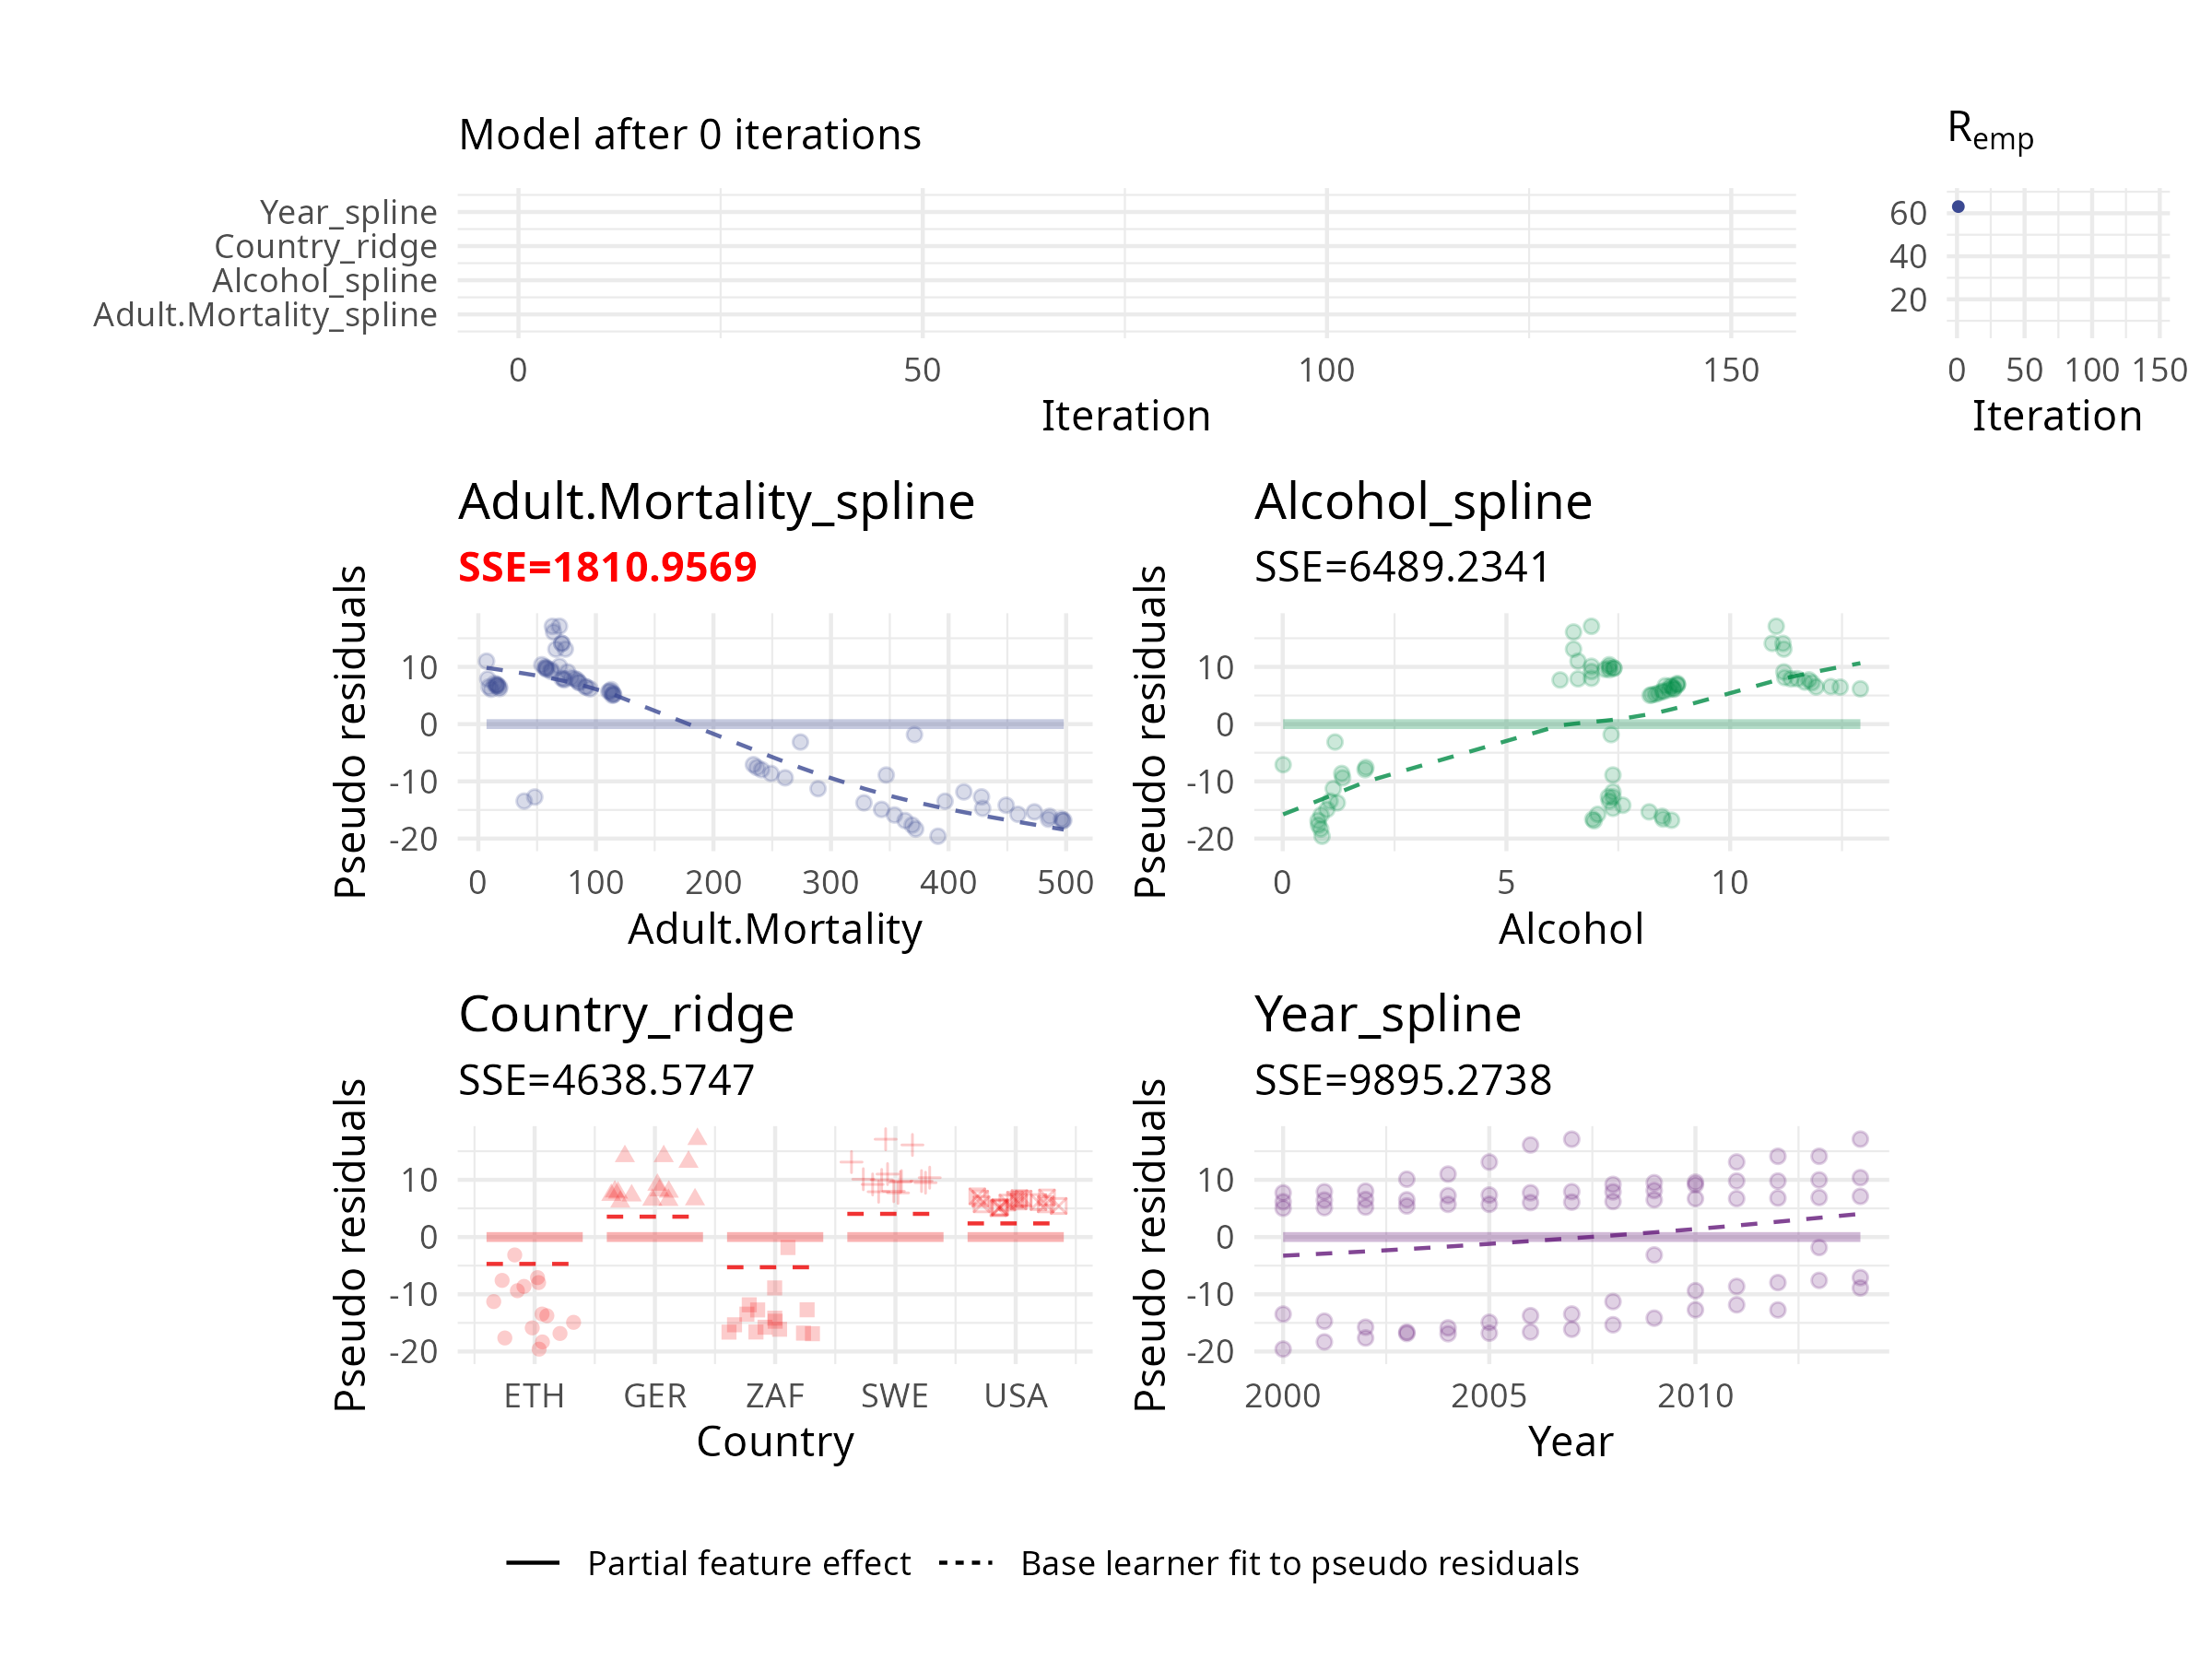
\includegraphics[width=\textwidth]{/home/daniel/repos/diss-presentation/figures/fig-iter-0001.png}
	\end{figure}
	\addtocounter{framenumber}{0}
\end{frame}


\begin{frame}{Component-wise gradient boosting -- Example}
	\begin{figure}
		\centering
		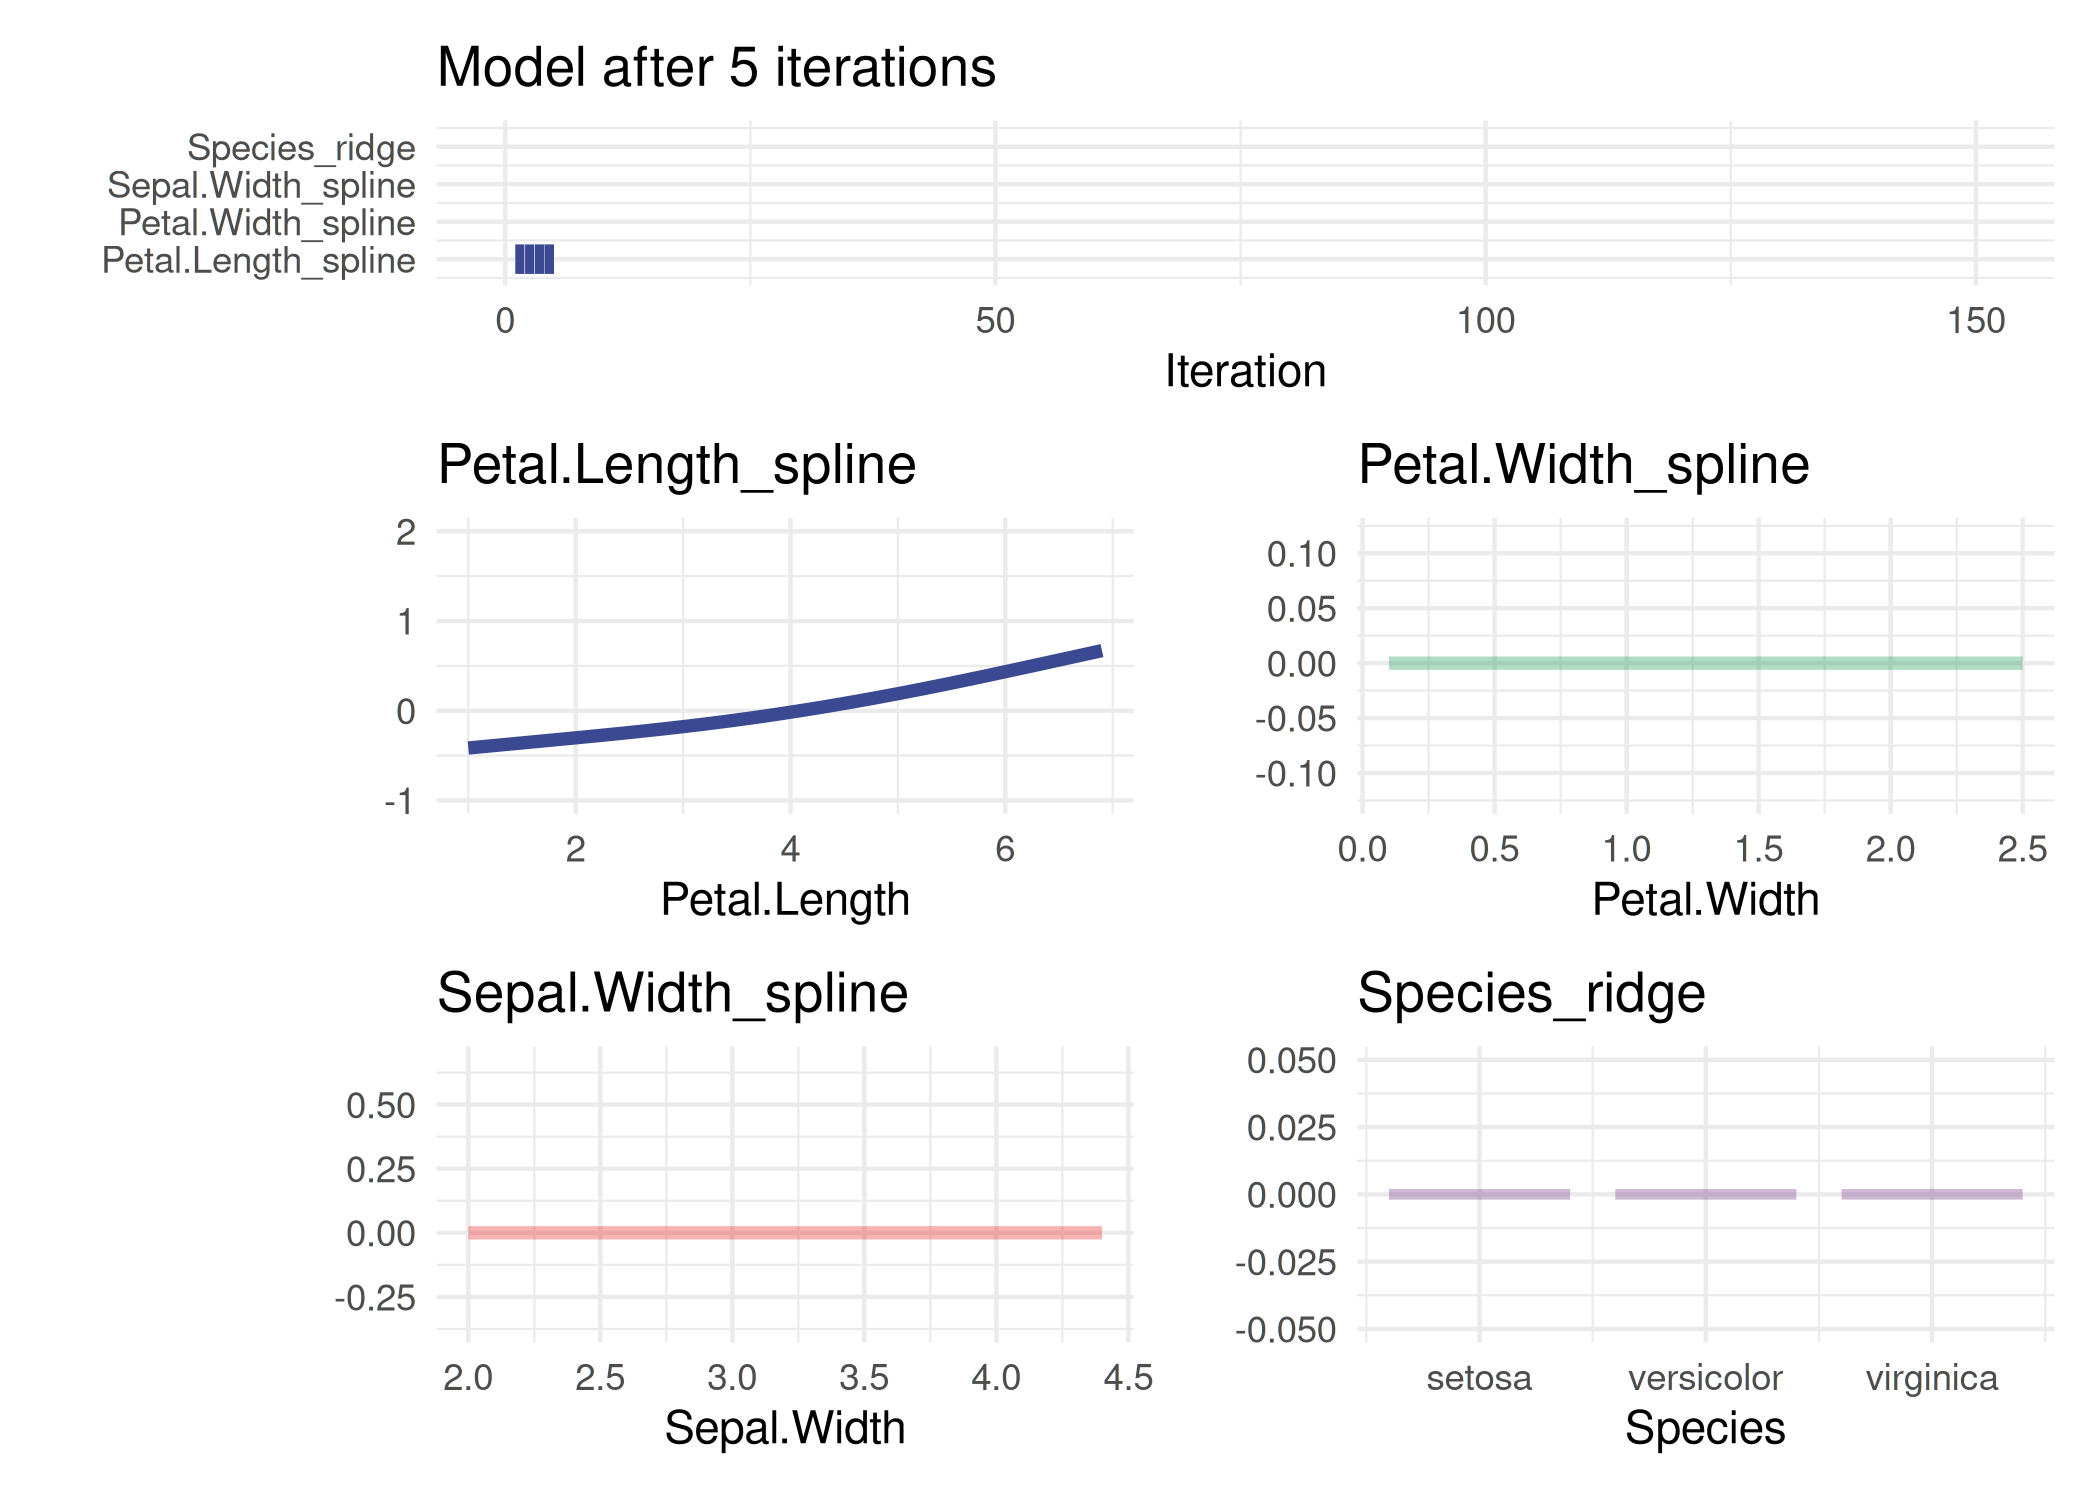
\includegraphics[width=\textwidth]{/home/daniel/repos/diss-presentation/figures/fig-iter-0005.png}
	\end{figure}
	\addtocounter{framenumber}{-1}
\end{frame}


\begin{frame}{Component-wise gradient boosting -- Example}
	\begin{figure}
		\centering
		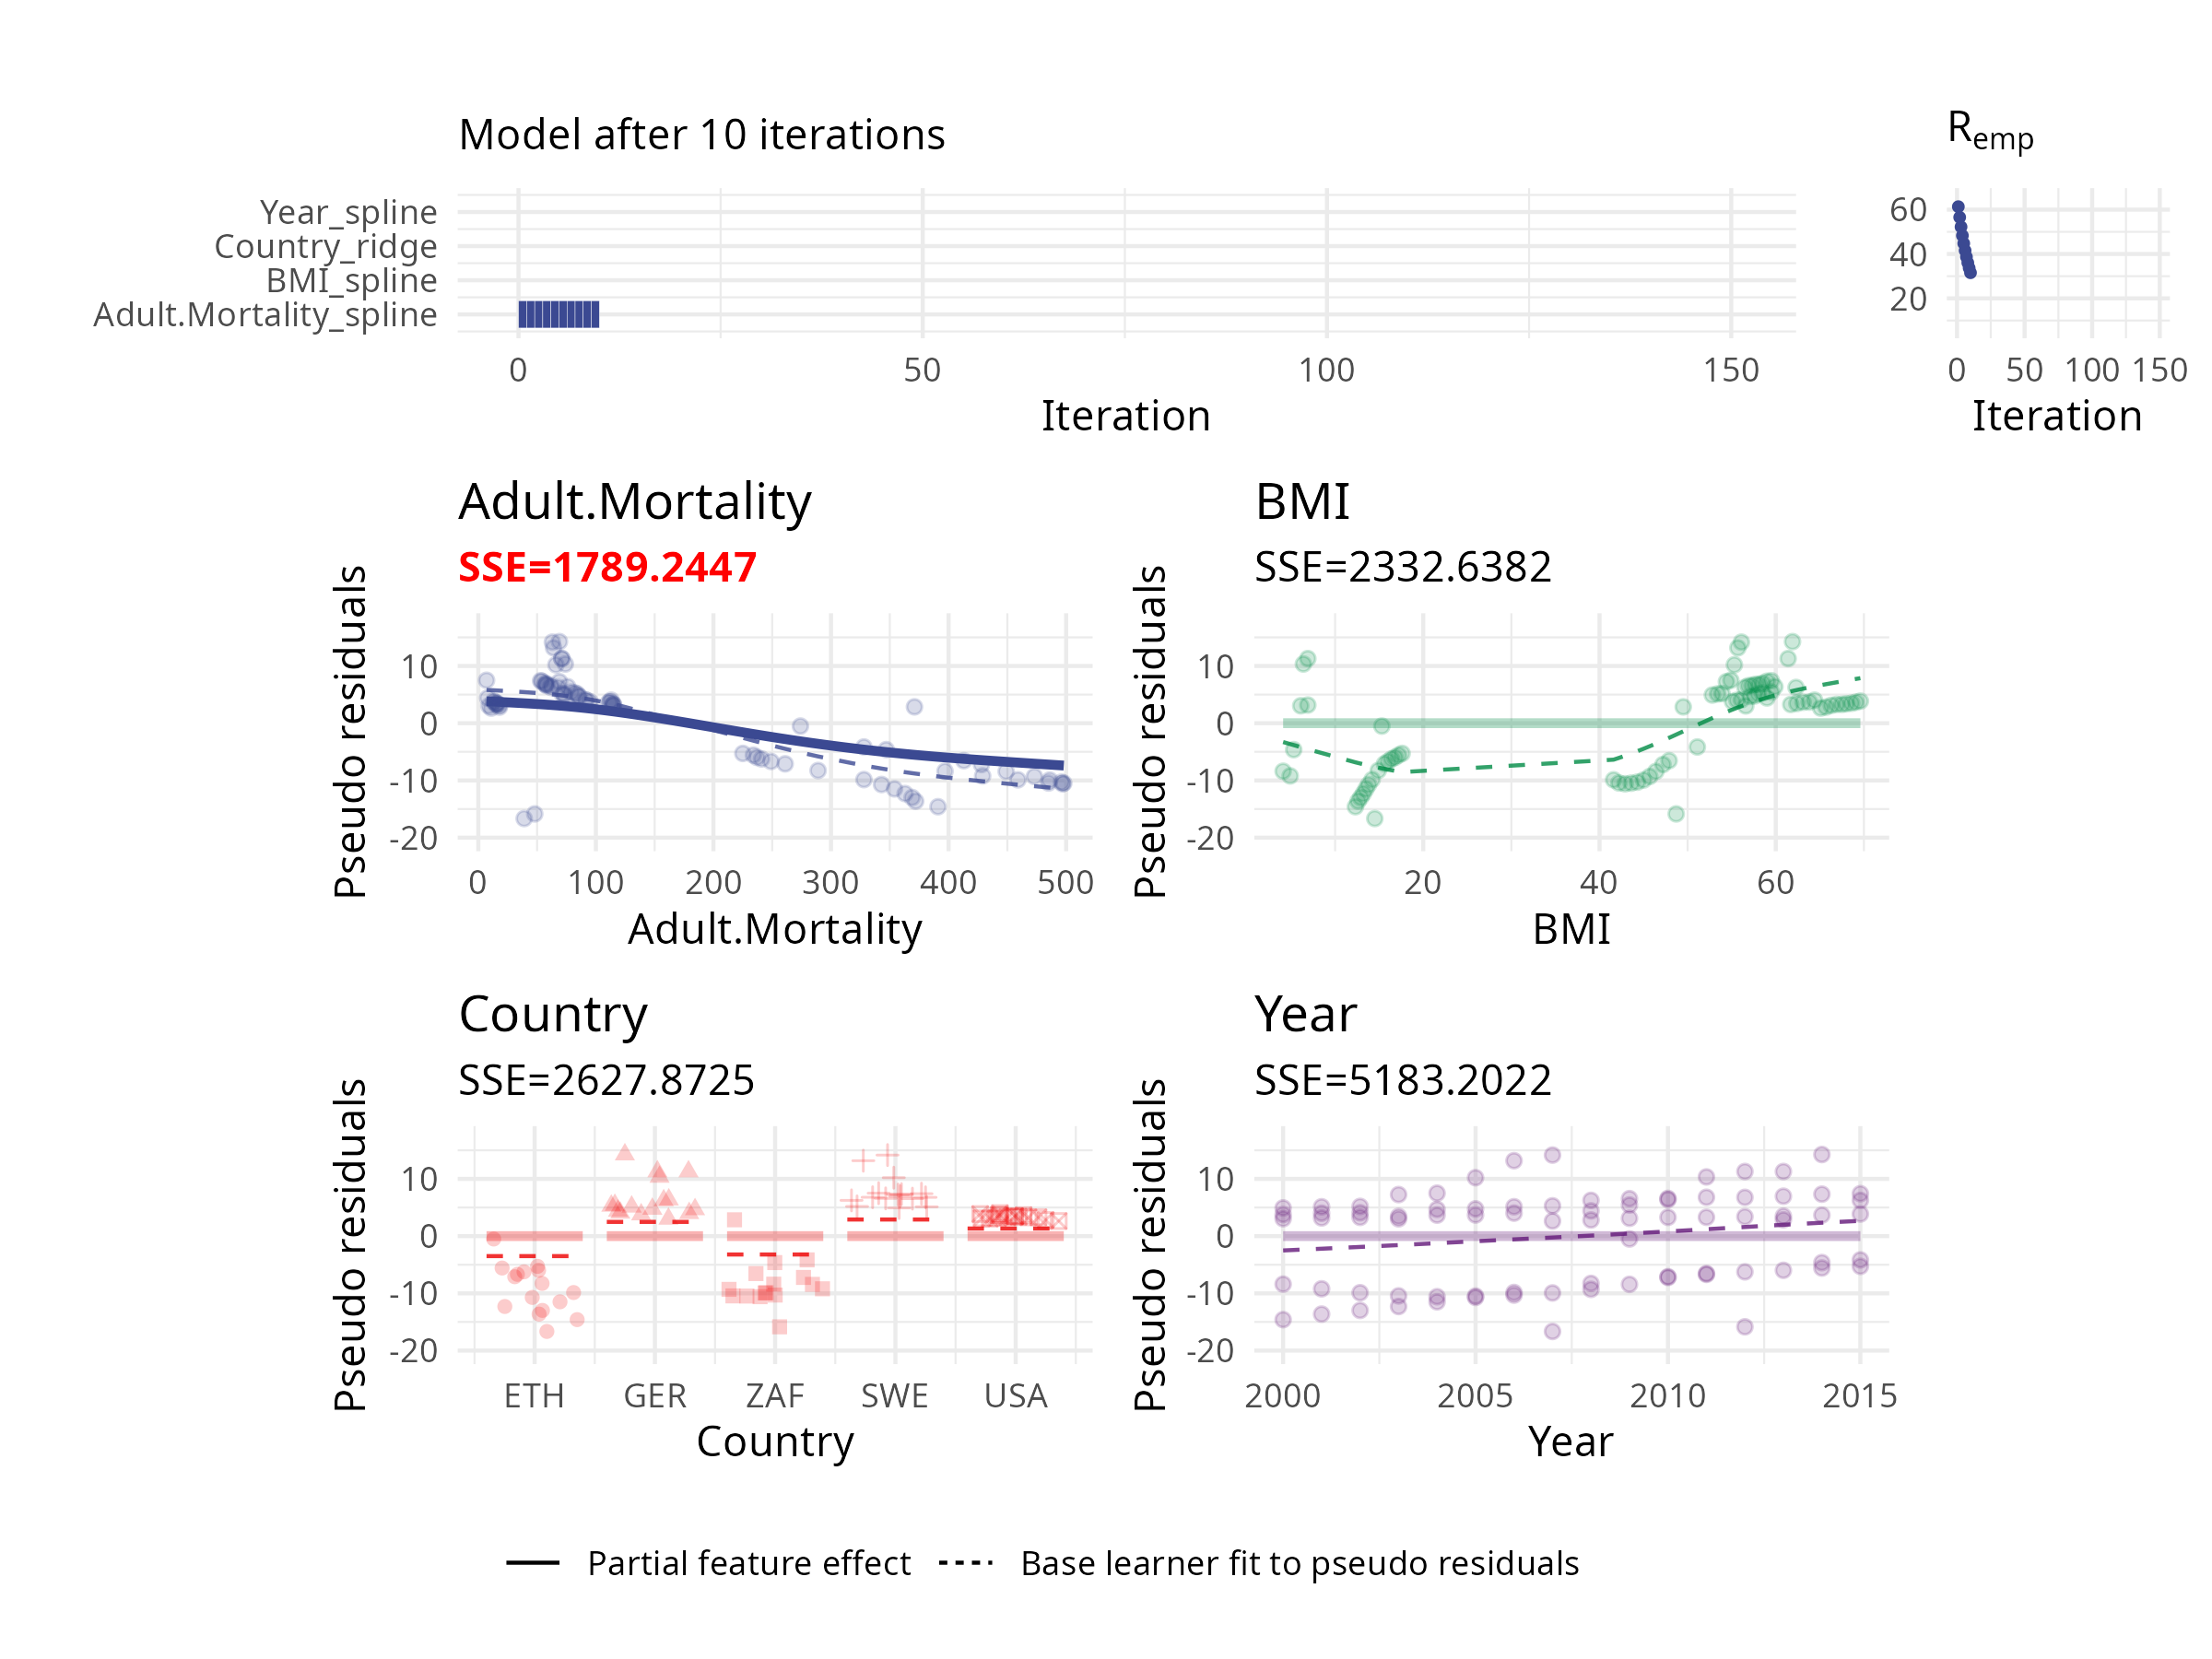
\includegraphics[width=\textwidth]{/home/daniel/repos/diss-presentation/figures/fig-iter-0010.png}
	\end{figure}
	\addtocounter{framenumber}{-1}
\end{frame}


\begin{frame}{Component-wise gradient boosting -- Example}
	\begin{figure}
		\centering
		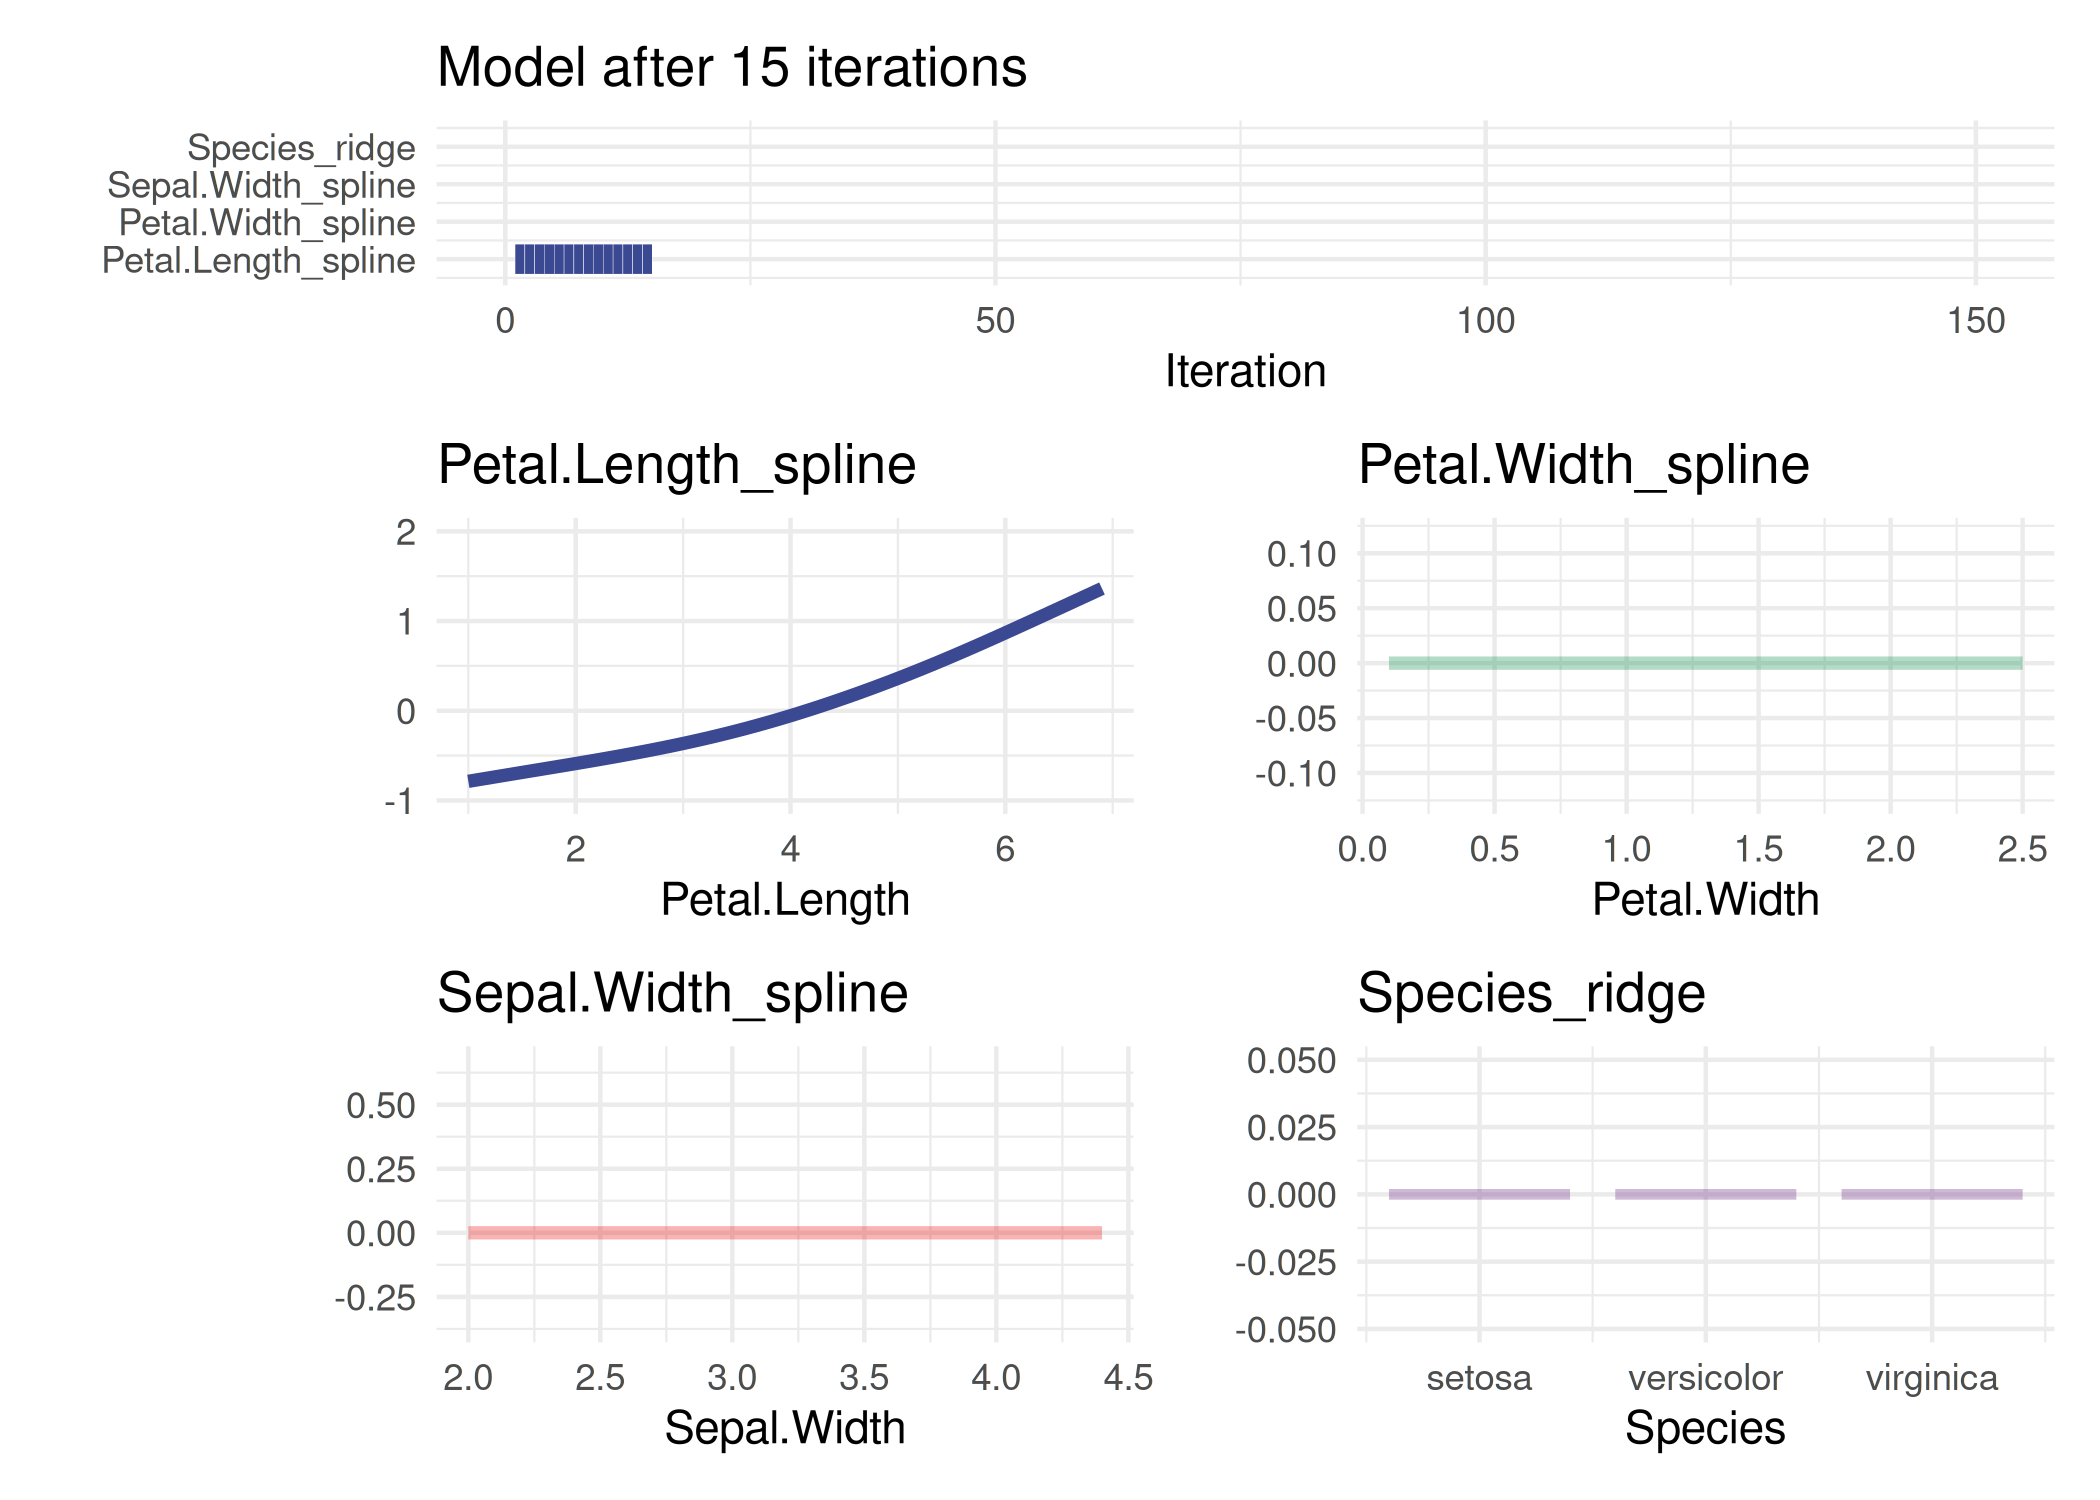
\includegraphics[width=\textwidth]{/home/daniel/repos/diss-presentation/figures/fig-iter-0015.png}
	\end{figure}
	\addtocounter{framenumber}{-1}
\end{frame}


\begin{frame}{Component-wise gradient boosting -- Example}
	\begin{figure}
		\centering
		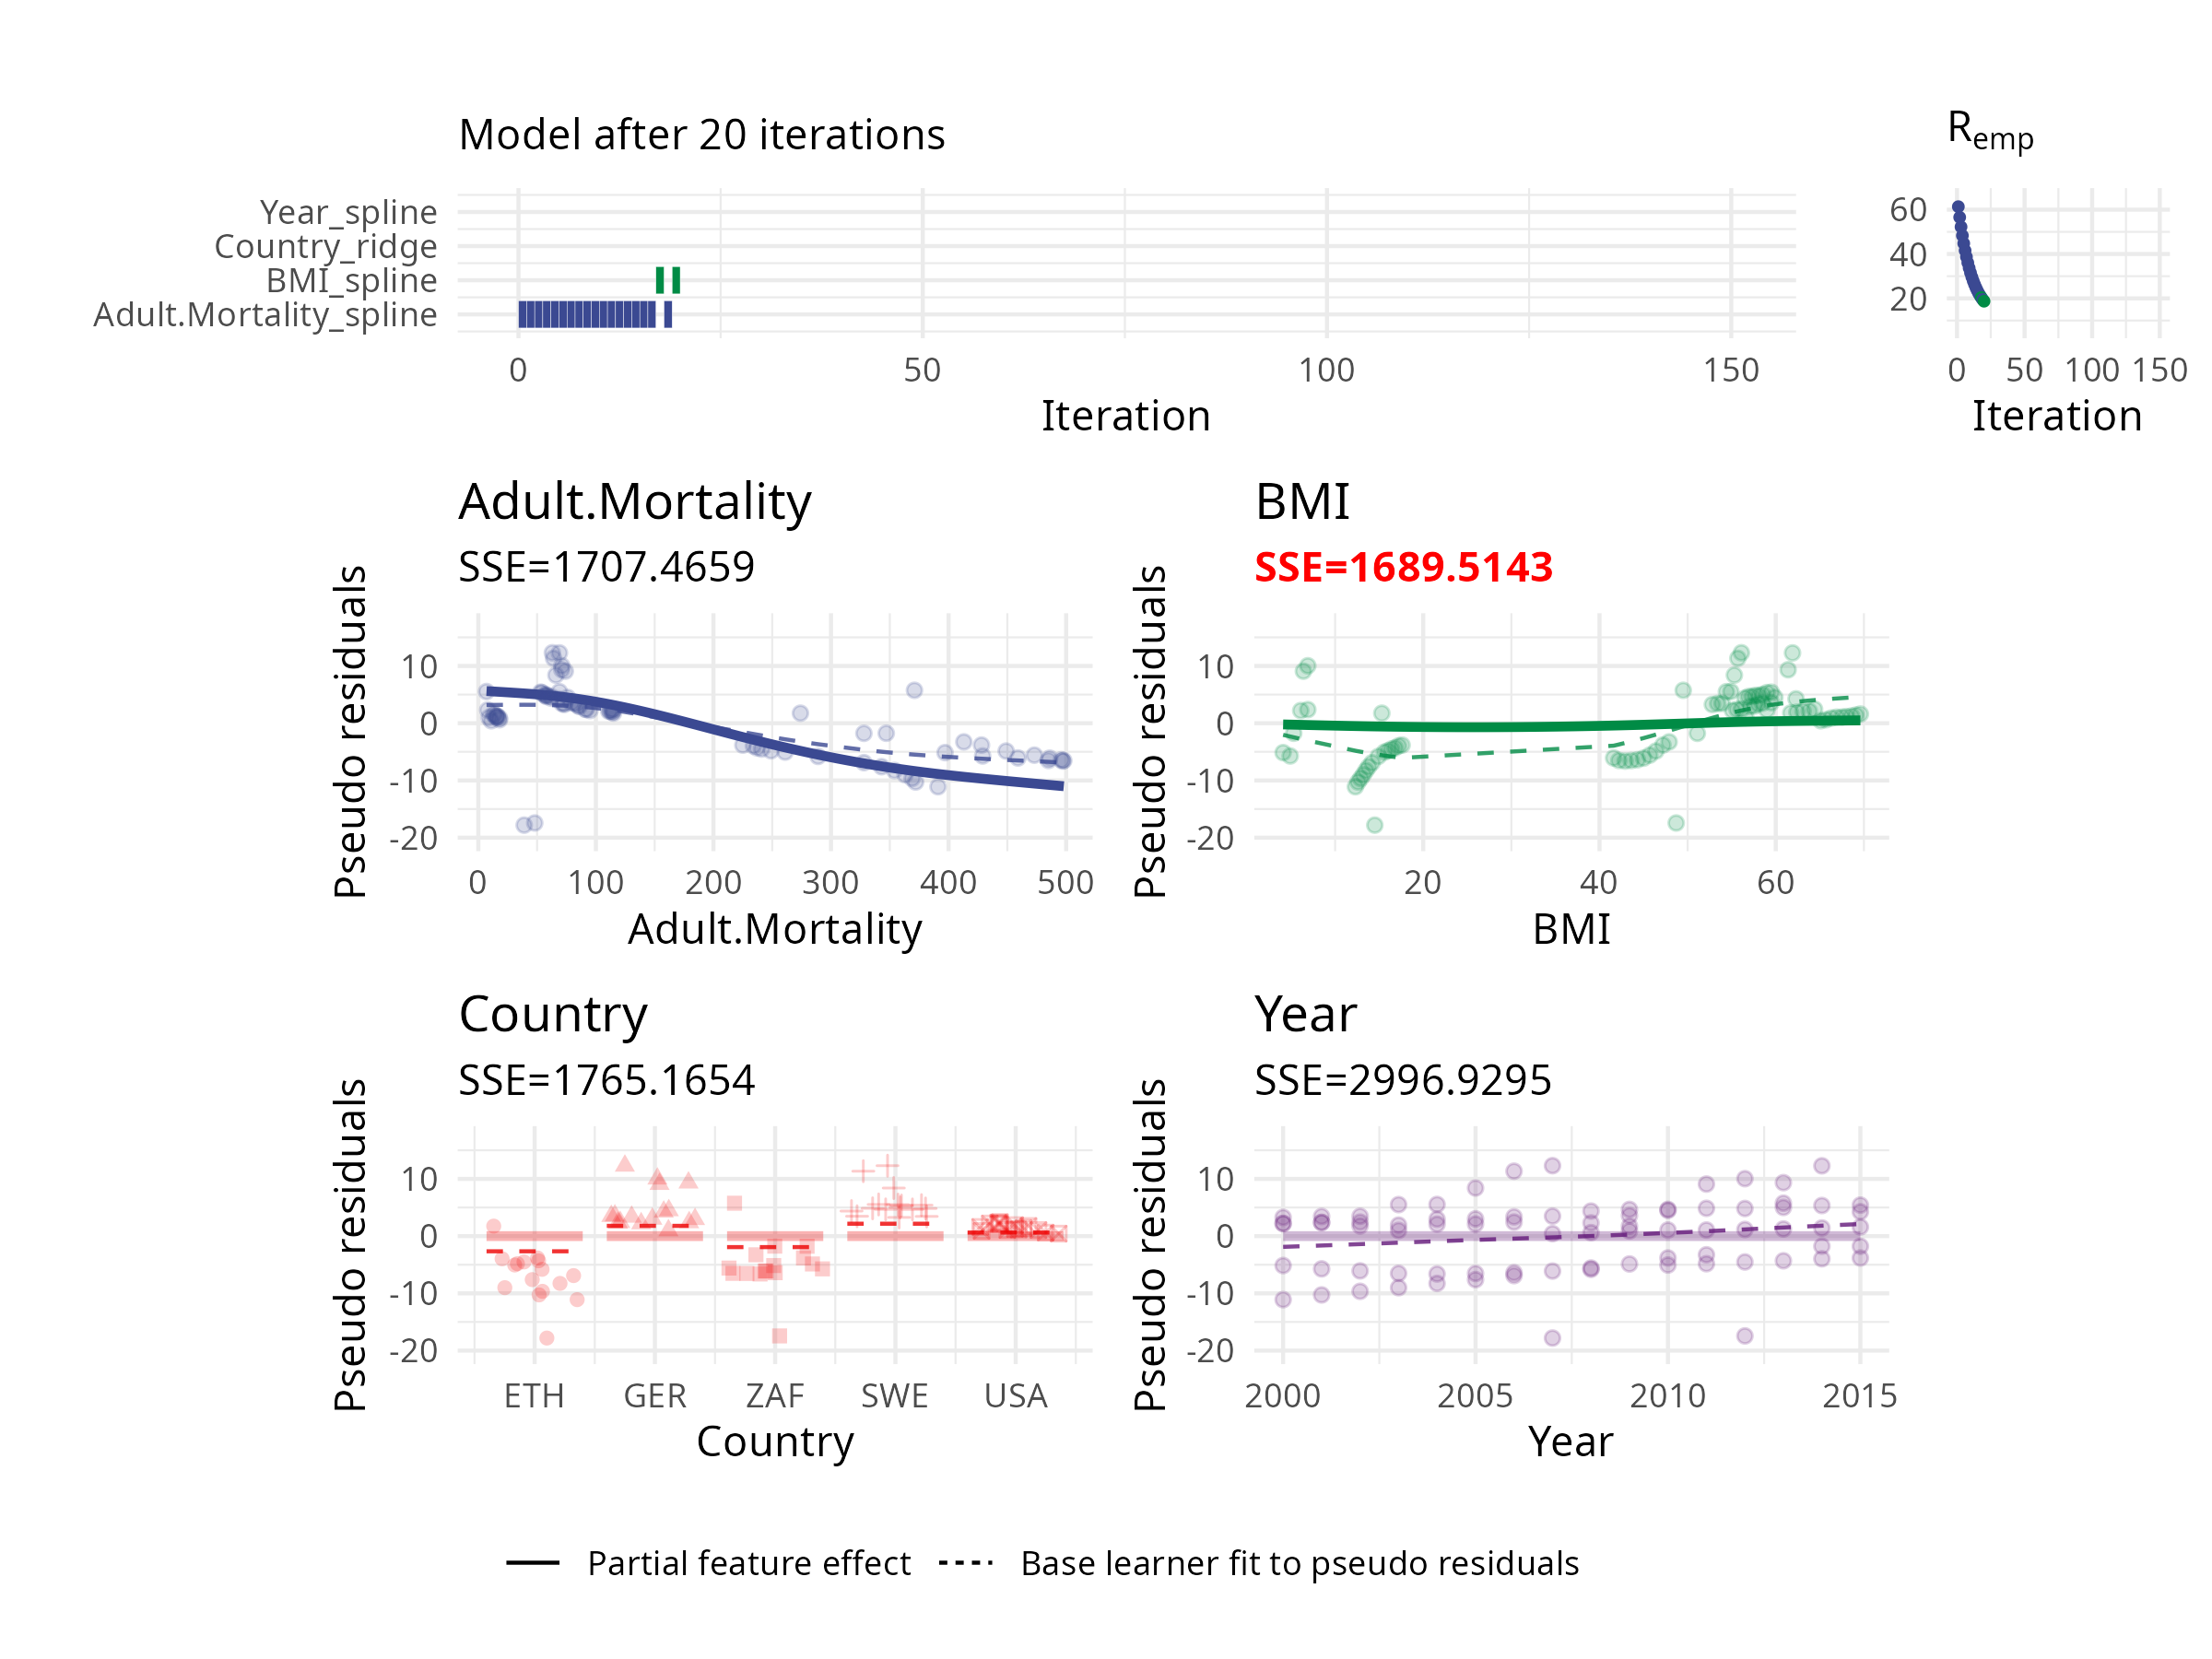
\includegraphics[width=\textwidth]{/home/daniel/repos/diss-presentation/figures/fig-iter-0020.png}
	\end{figure}
	\addtocounter{framenumber}{-1}
\end{frame}


\begin{frame}{Component-wise gradient boosting -- Example}
	\begin{figure}
		\centering
		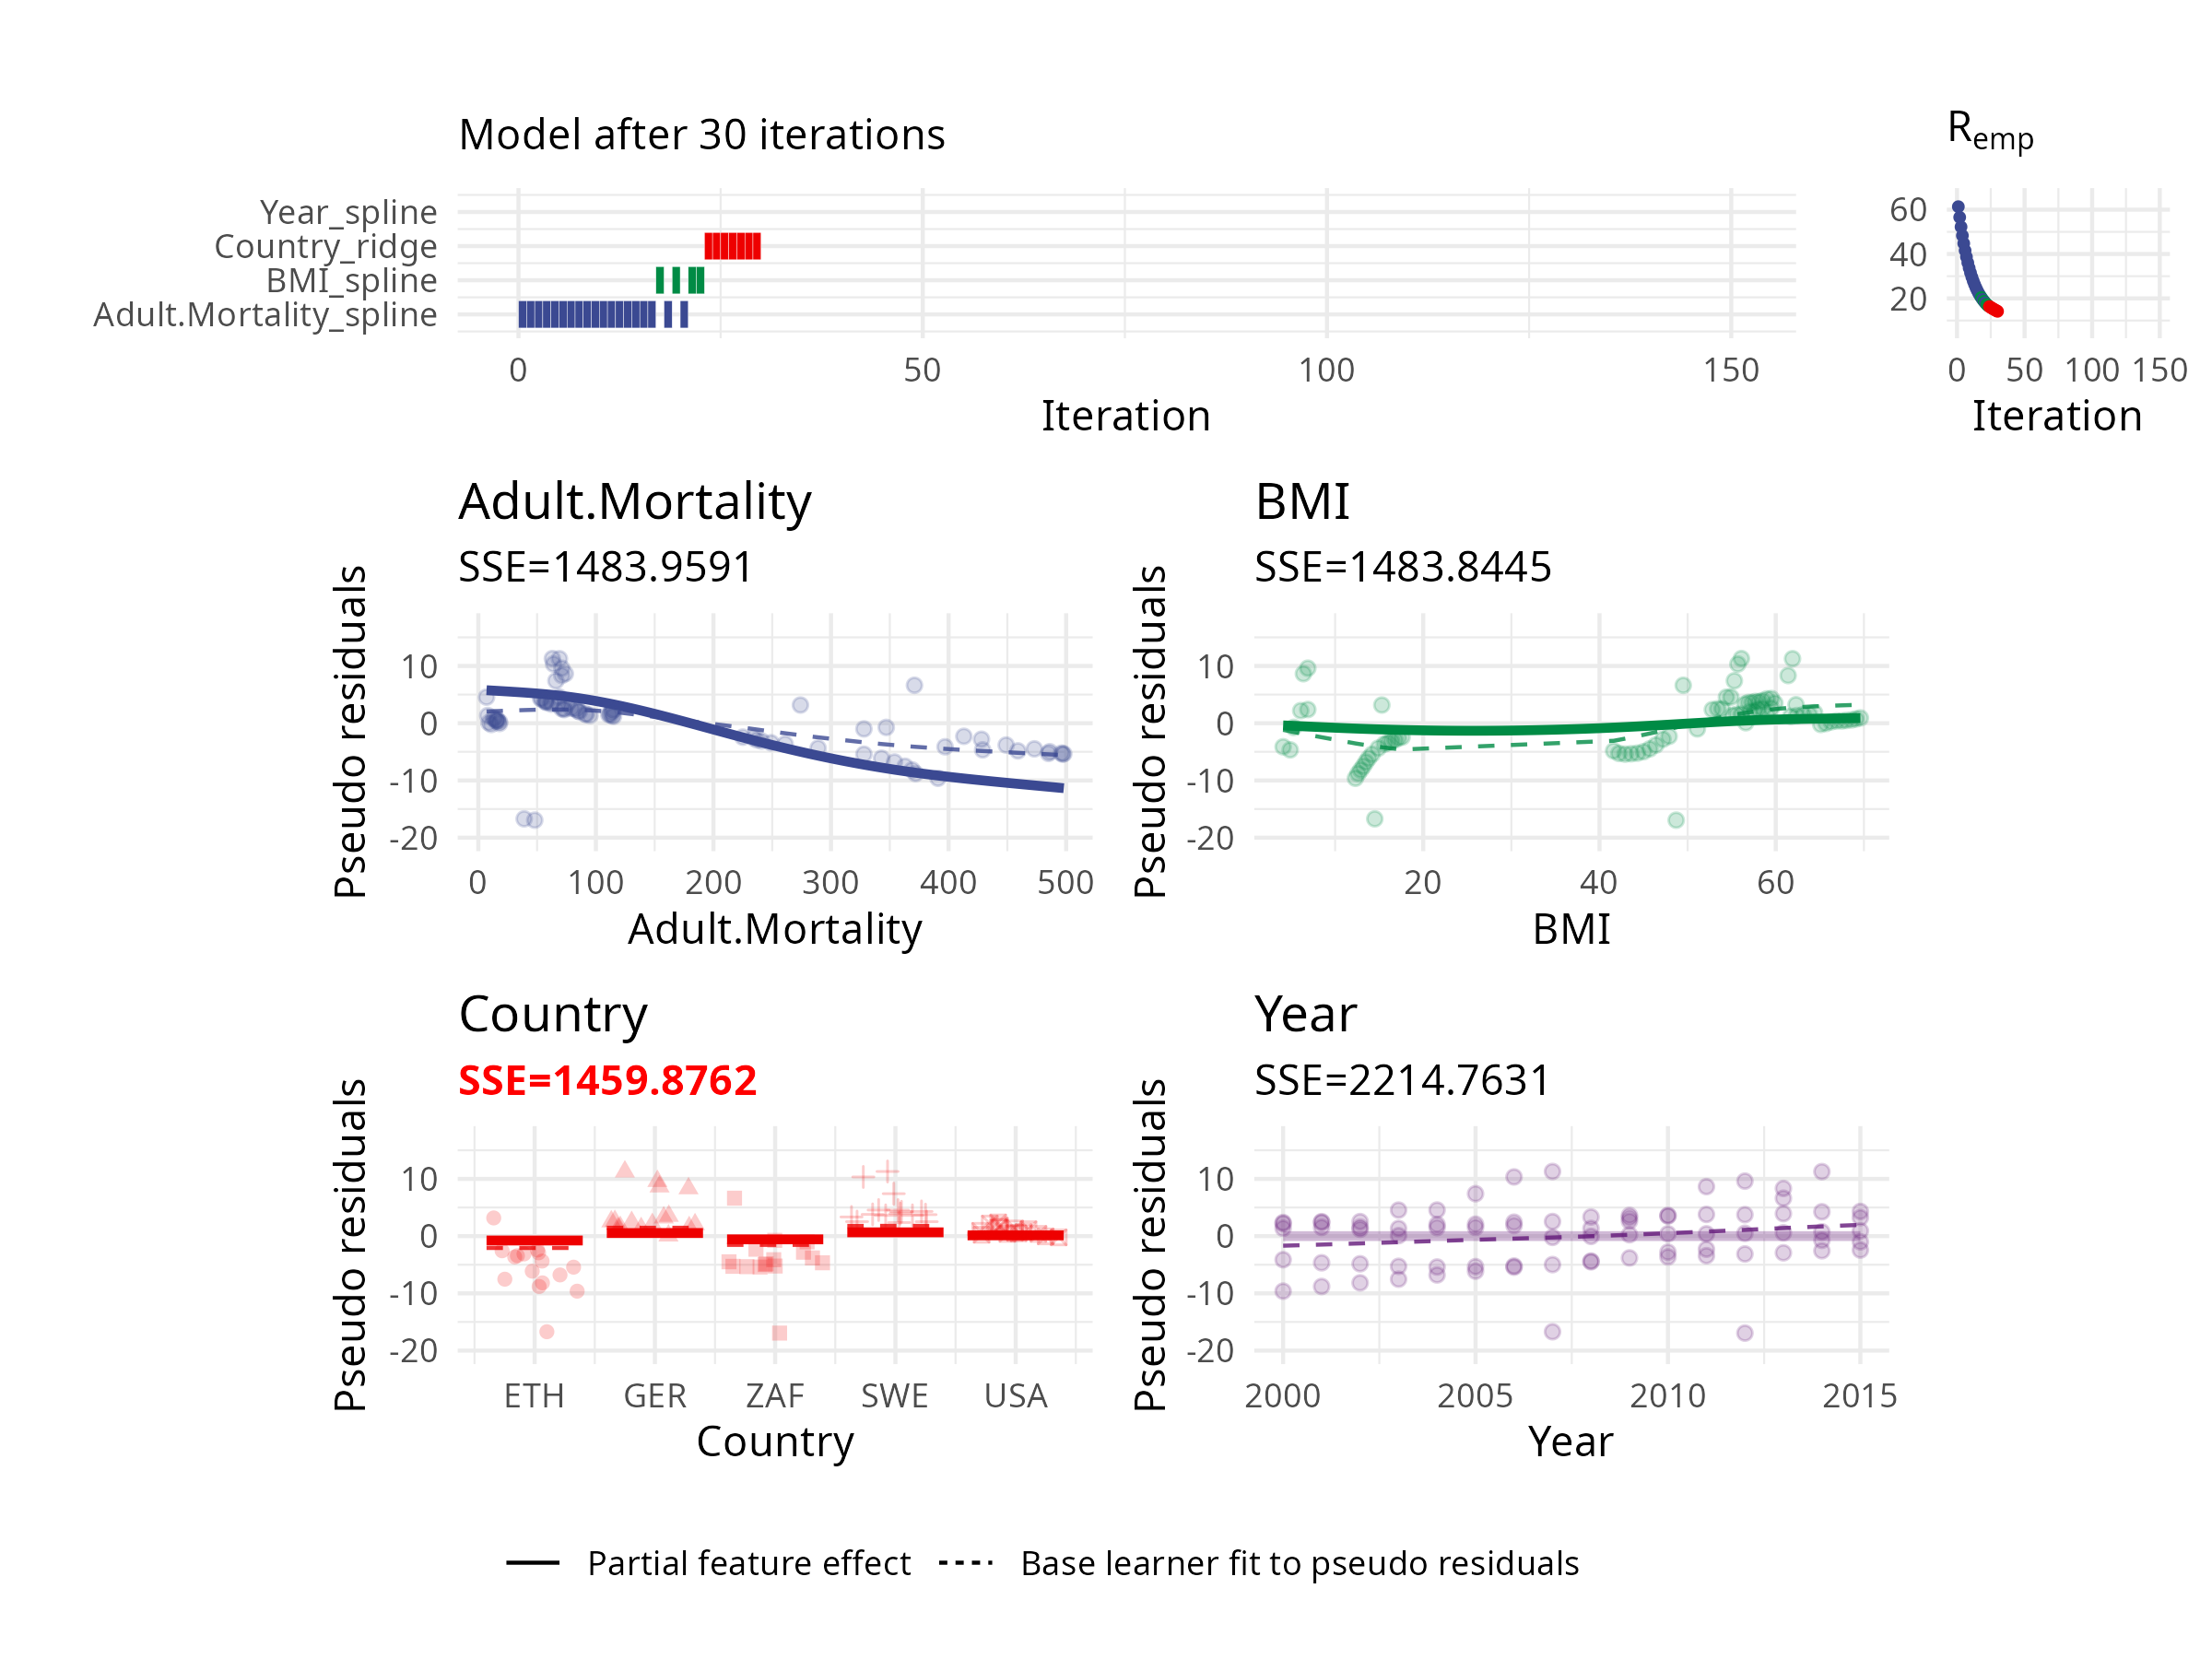
\includegraphics[width=\textwidth]{/home/daniel/repos/diss-presentation/figures/fig-iter-0030.png}
	\end{figure}
	\addtocounter{framenumber}{-1}
\end{frame}


\begin{frame}{Component-wise gradient boosting -- Example}
	\begin{figure}
		\centering
		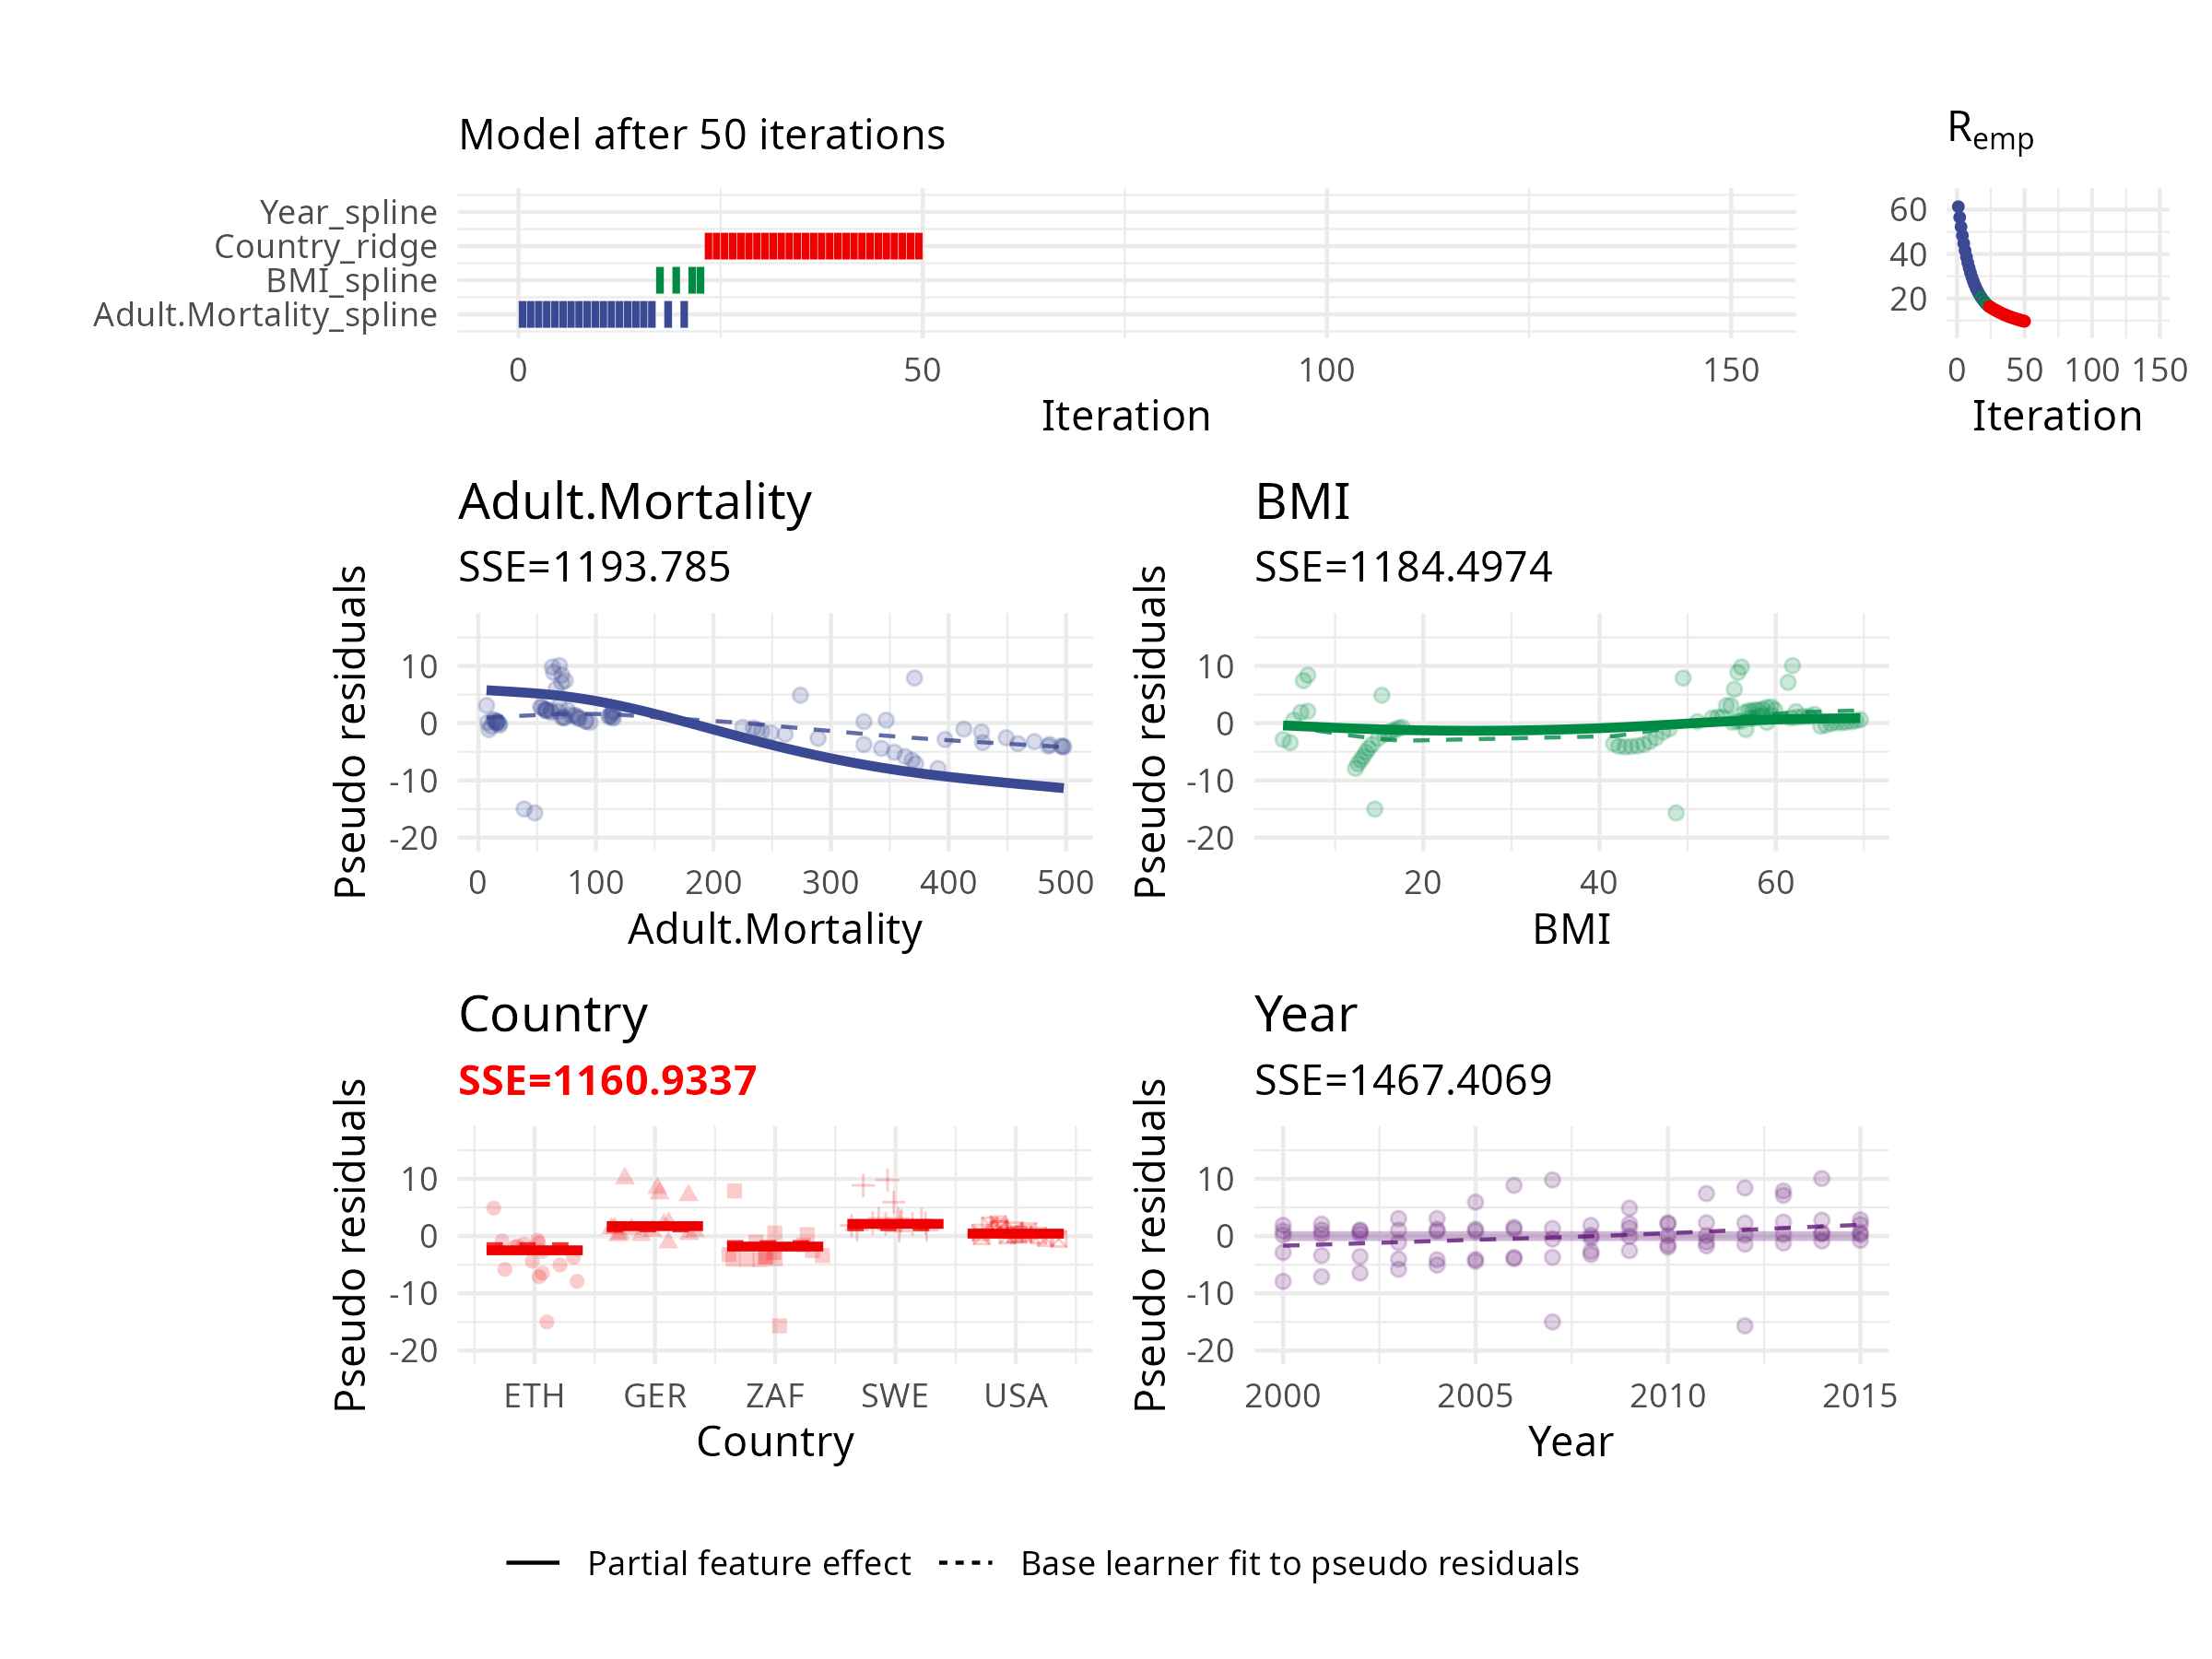
\includegraphics[width=\textwidth]{/home/daniel/repos/diss-presentation/figures/fig-iter-0050.png}
	\end{figure}
	\addtocounter{framenumber}{-1}
\end{frame}


\begin{frame}{Component-wise gradient boosting -- Example}
	\begin{figure}
		\centering
		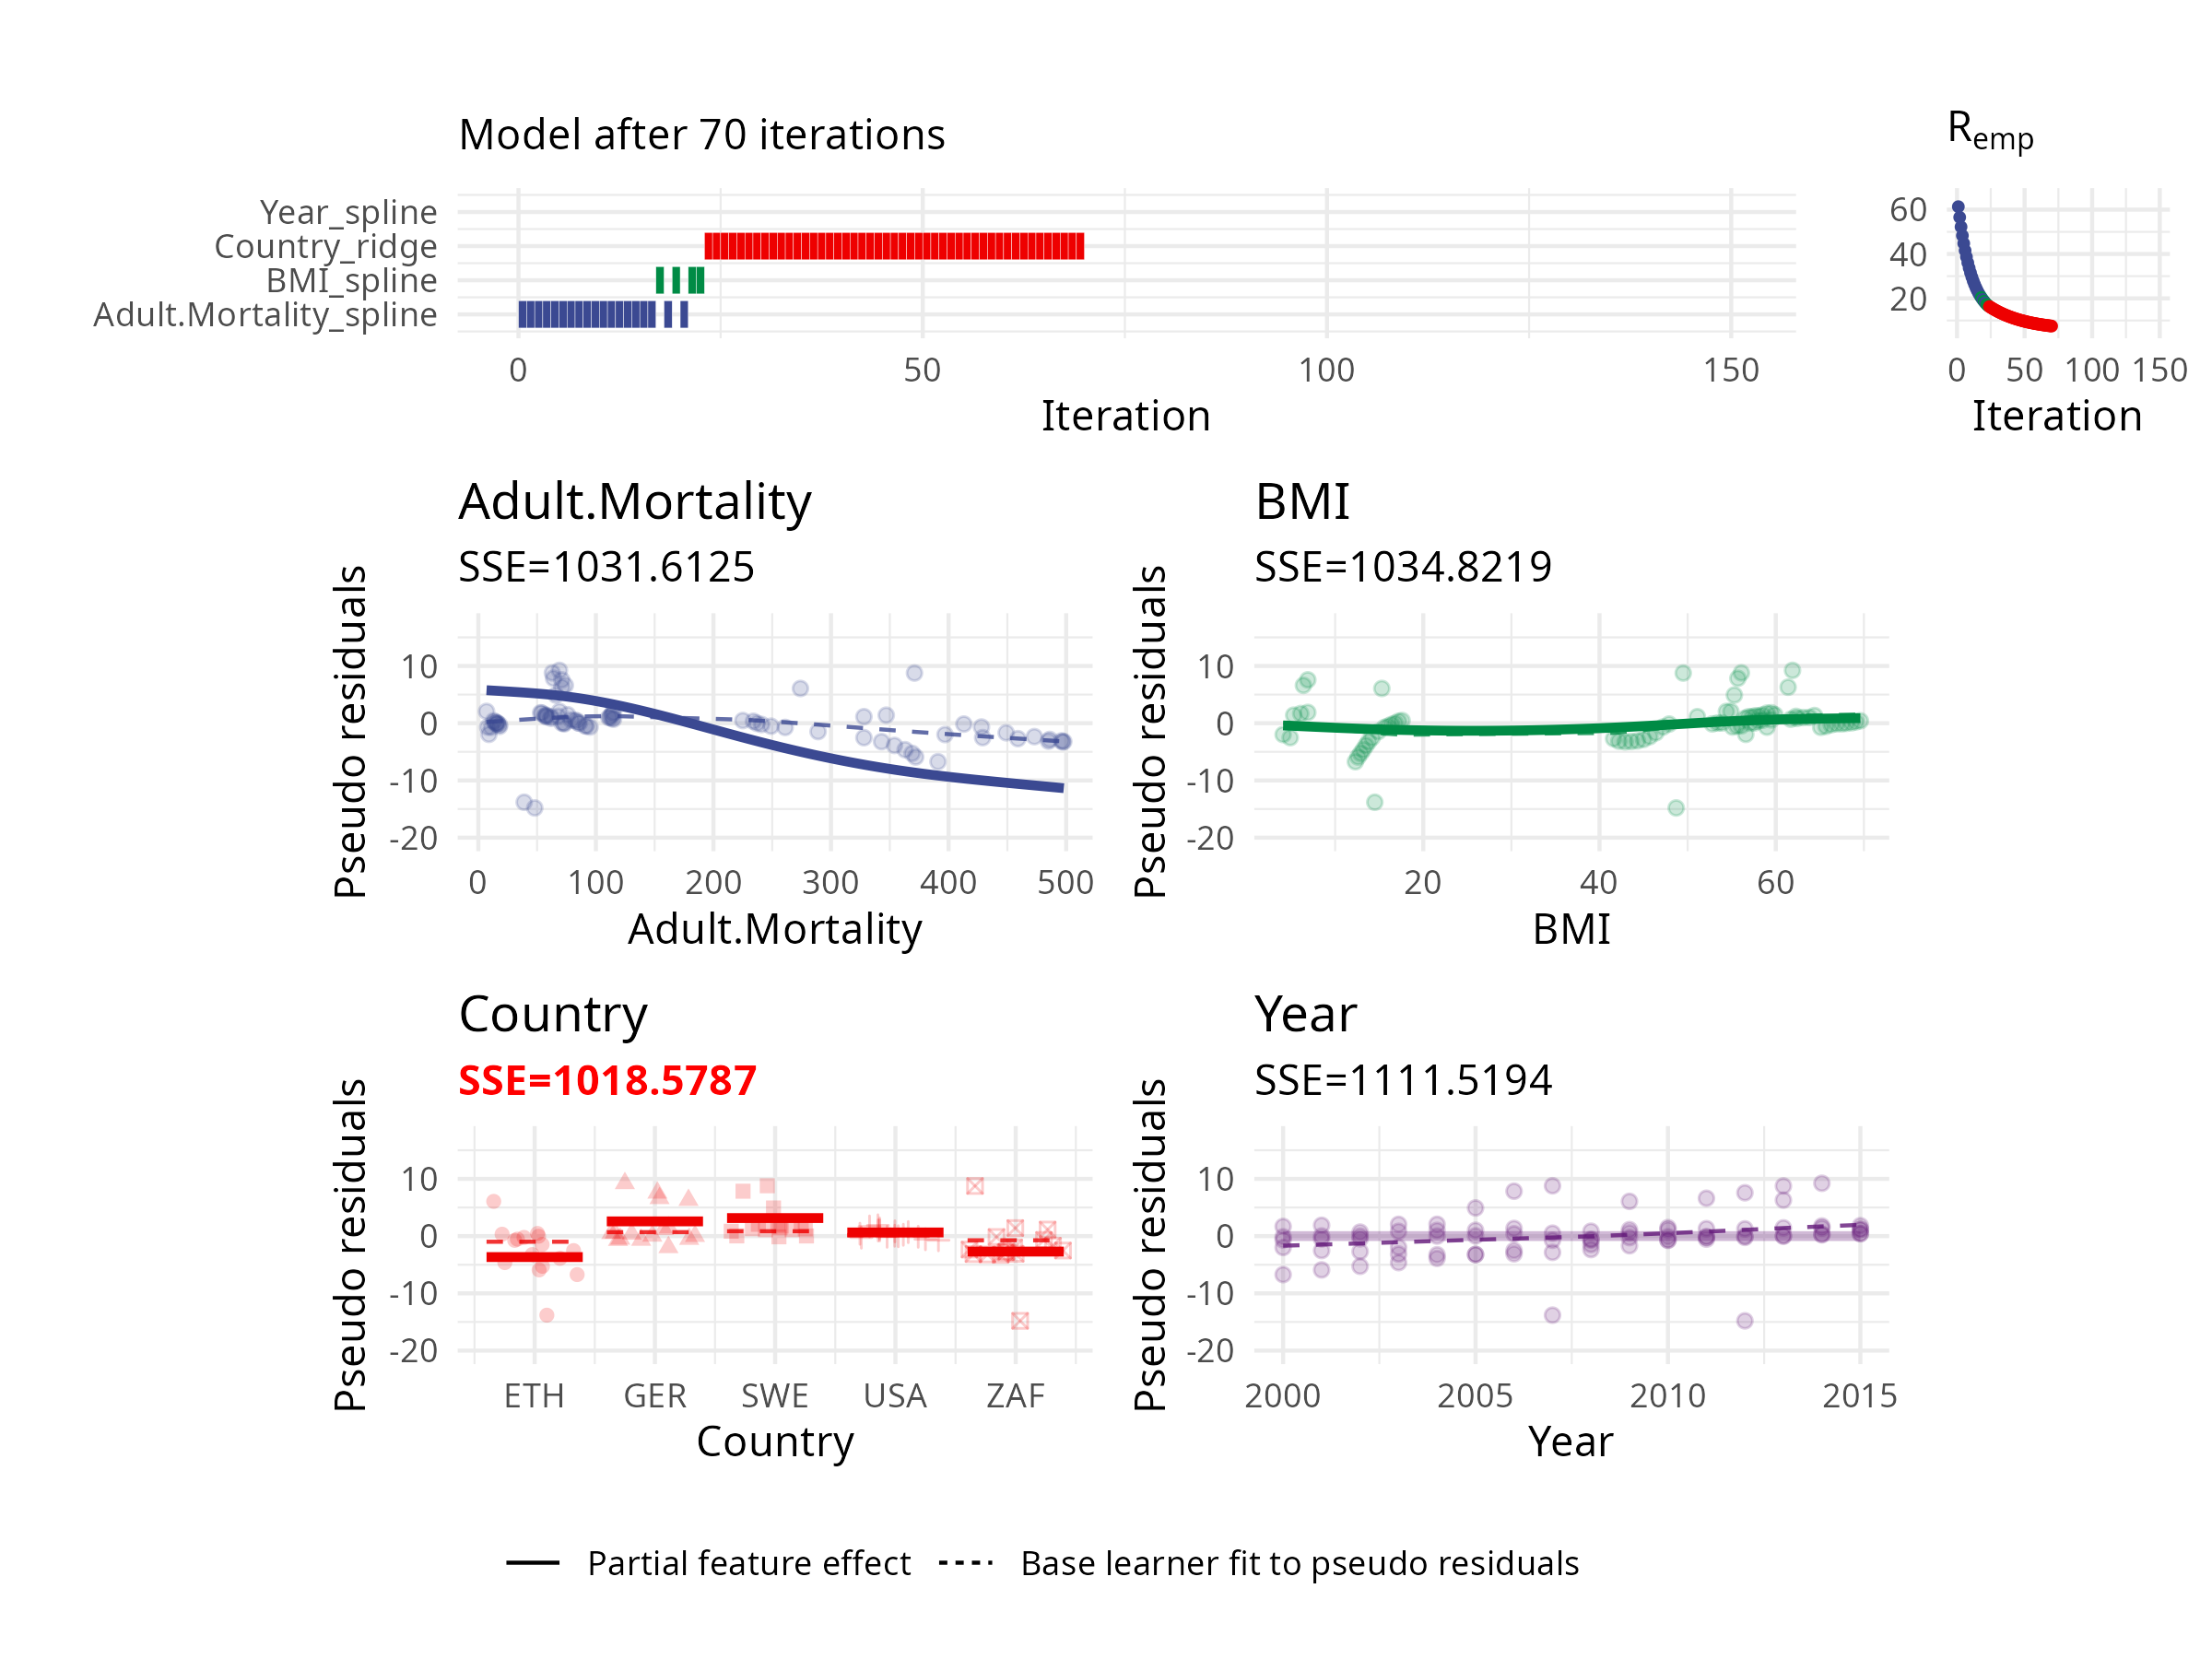
\includegraphics[width=\textwidth]{/home/daniel/repos/diss-presentation/figures/fig-iter-0070.png}
	\end{figure}
	\addtocounter{framenumber}{-1}
\end{frame}


\begin{frame}{Component-wise gradient boosting -- Example}
	\begin{figure}
		\centering
		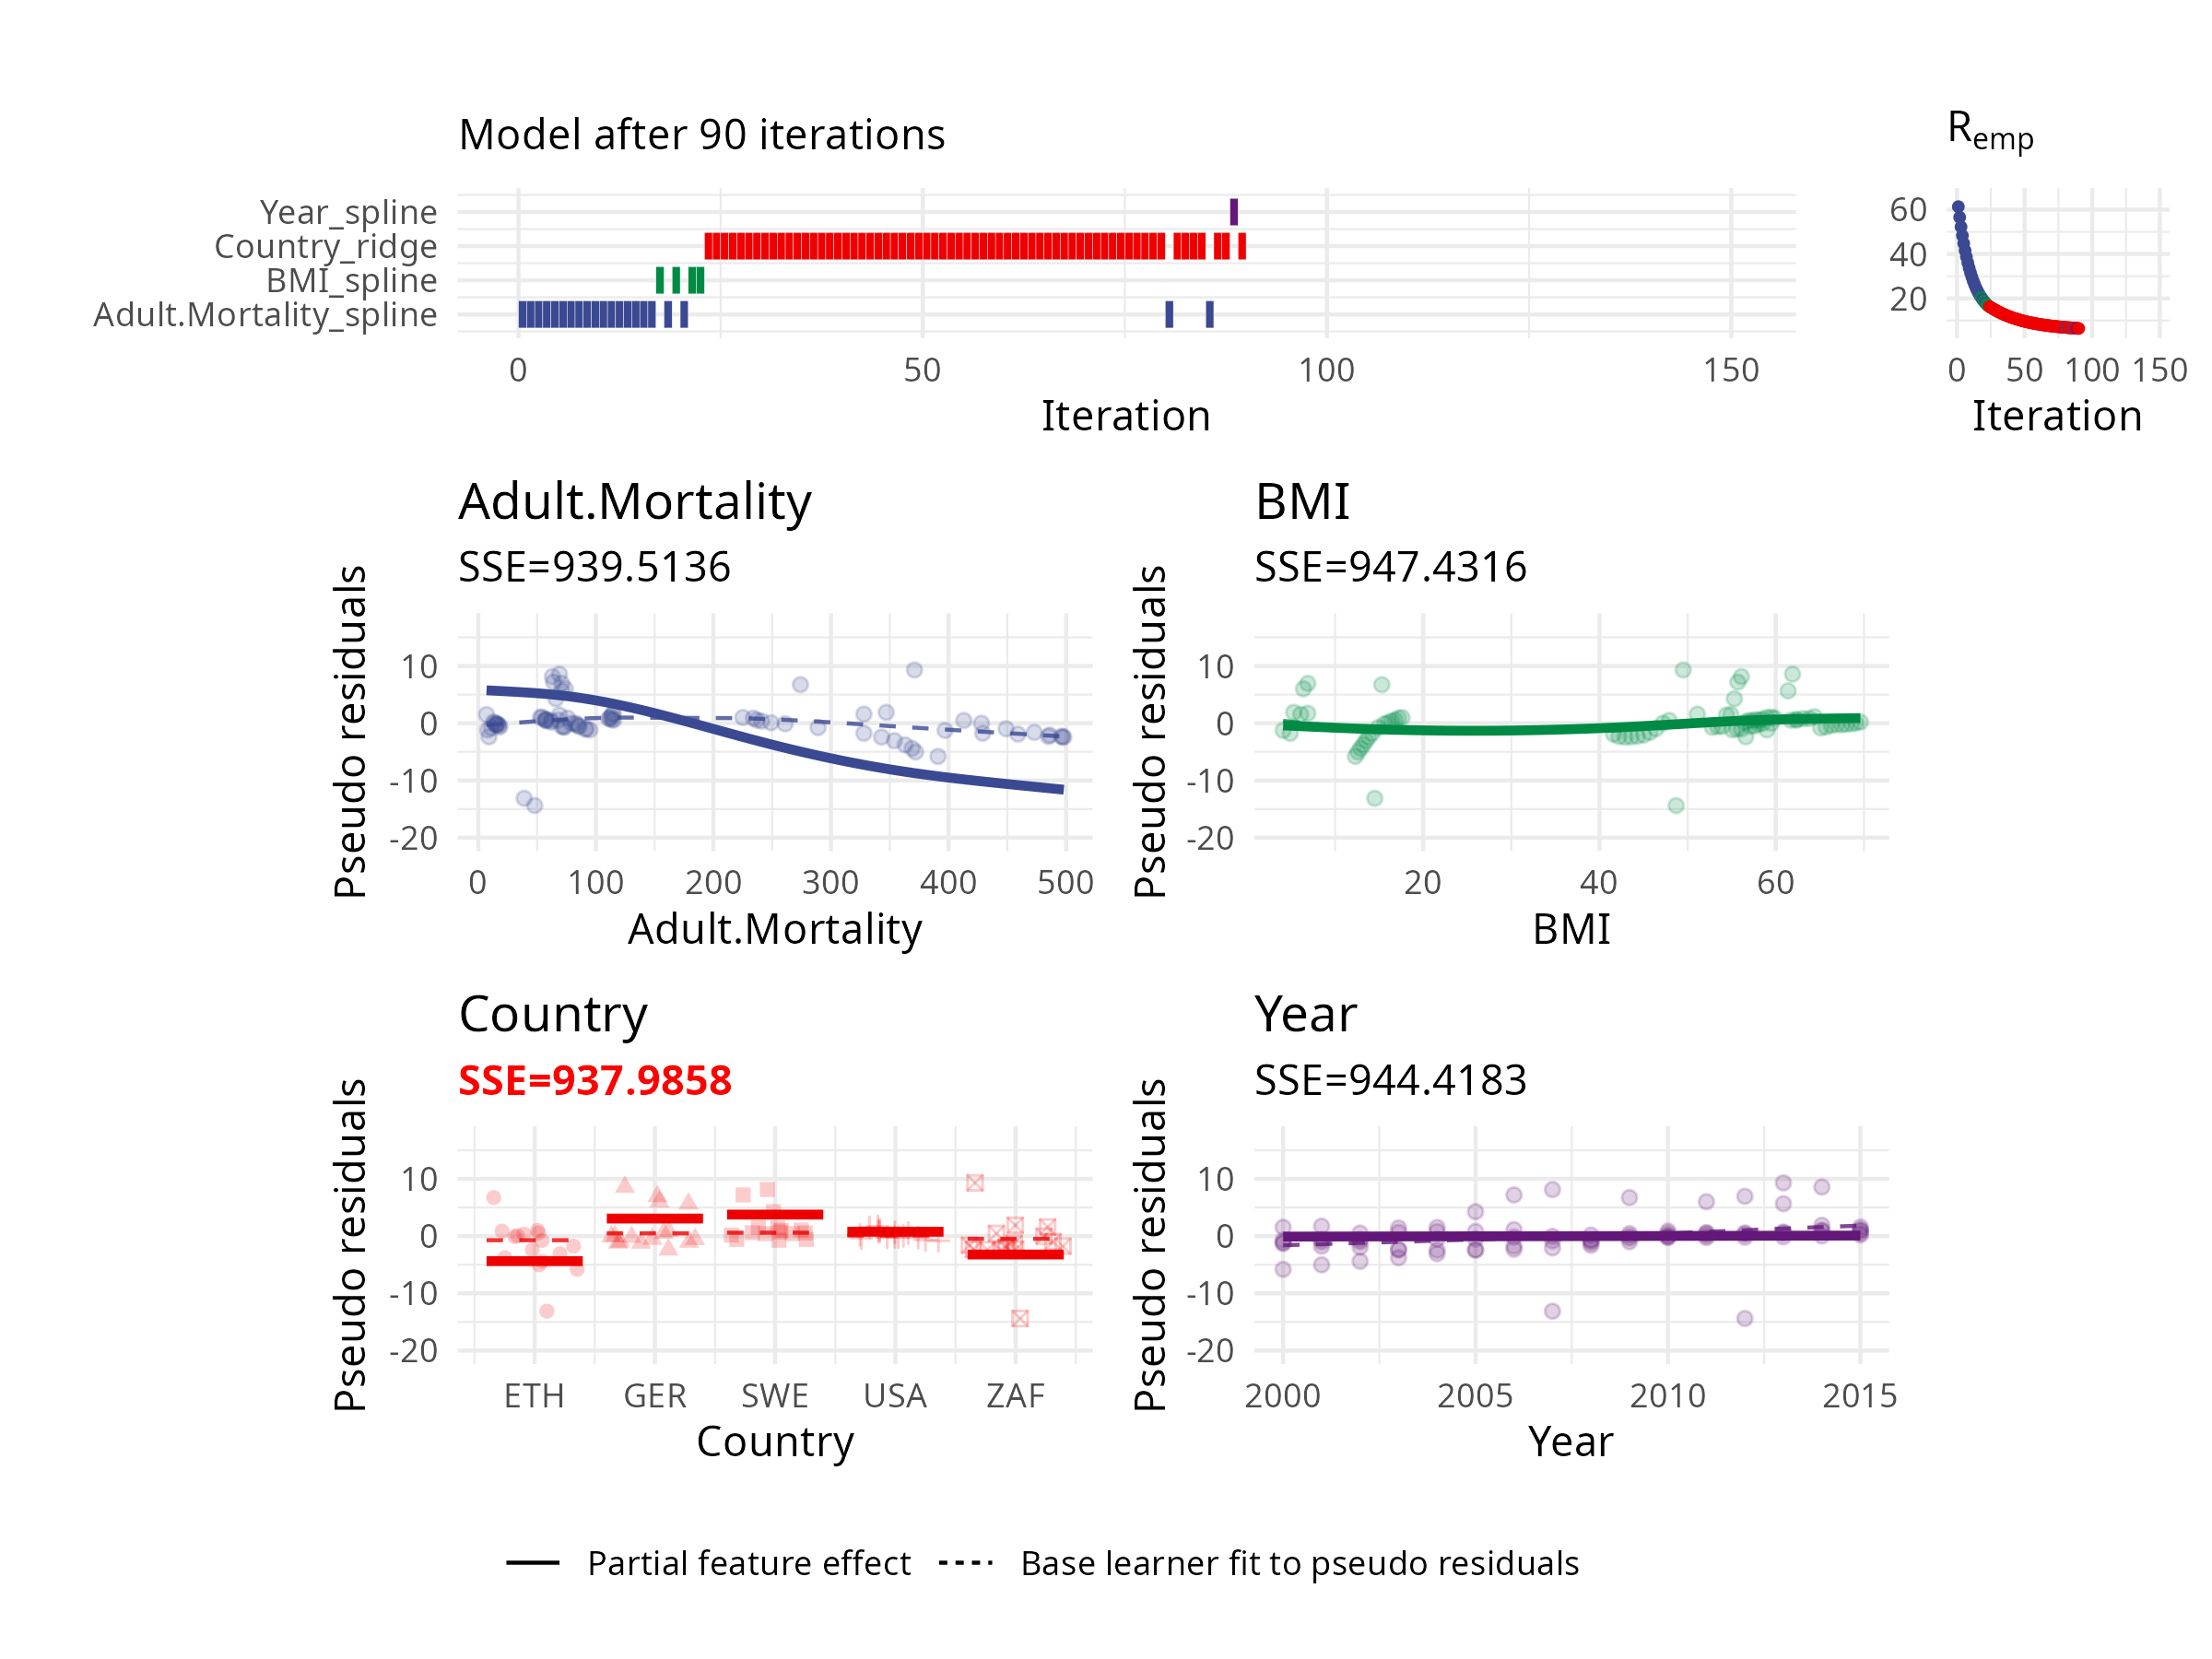
\includegraphics[width=\textwidth]{/home/daniel/repos/diss-presentation/figures/fig-iter-0090.png}
	\end{figure}
	\addtocounter{framenumber}{-1}
\end{frame}


\begin{frame}{Component-wise gradient boosting -- Example}
	\begin{figure}
		\centering
		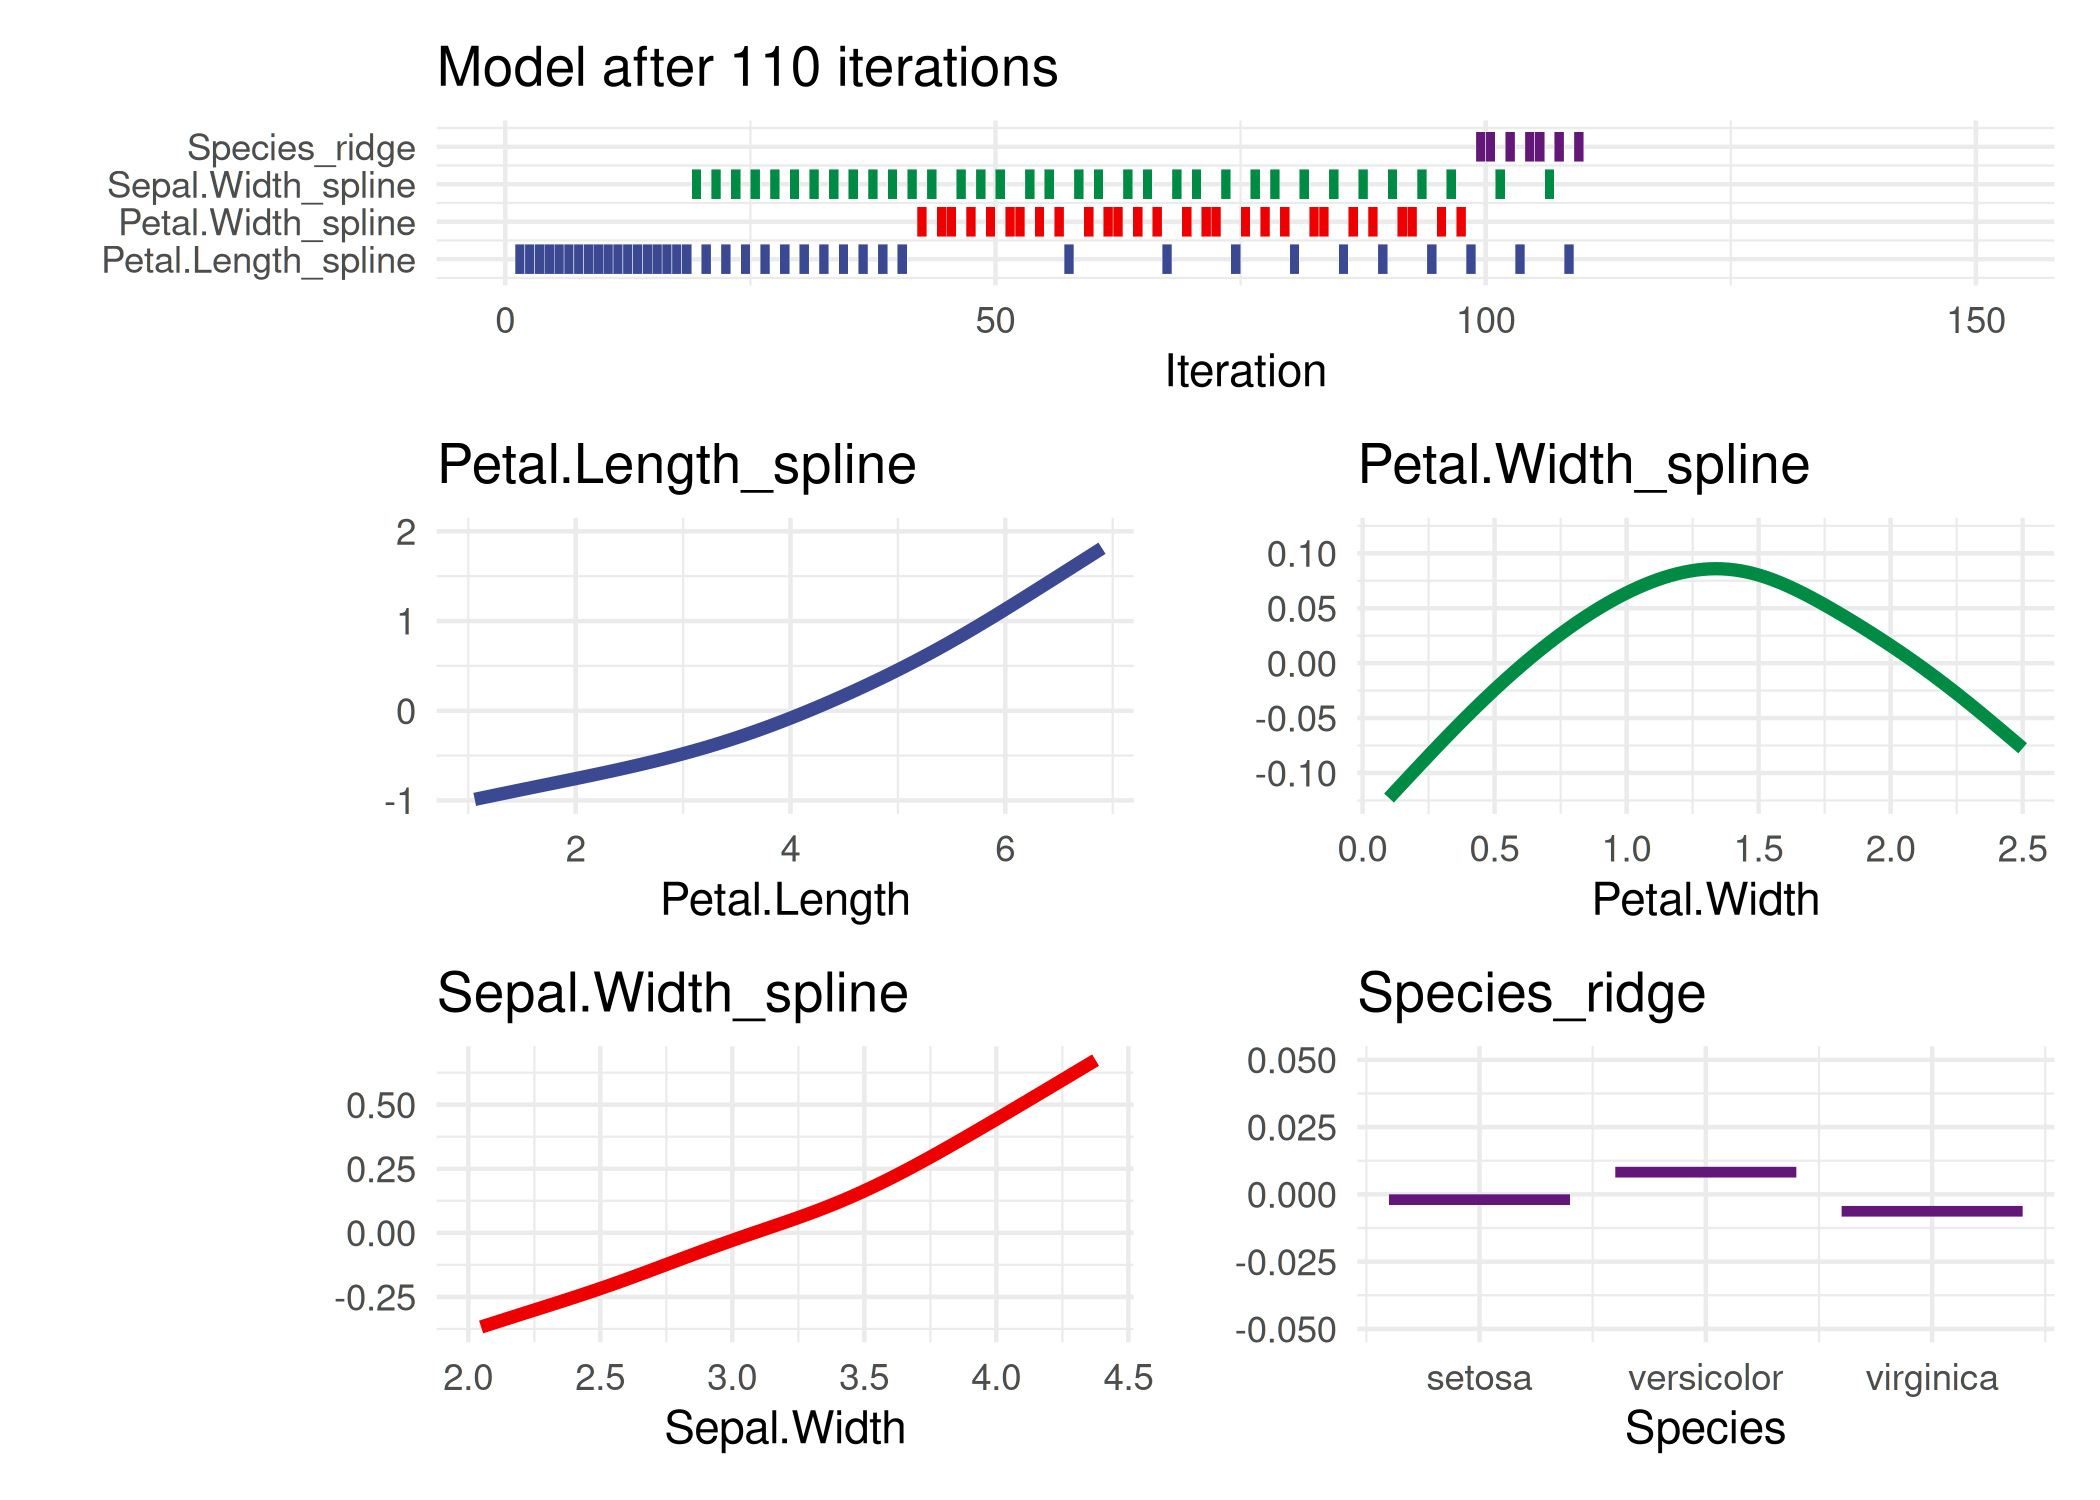
\includegraphics[width=\textwidth]{/home/daniel/repos/diss-presentation/figures/fig-iter-0110.png}
	\end{figure}
	\addtocounter{framenumber}{-1}
\end{frame}


\begin{frame}{Component-wise gradient boosting -- Example}
	\begin{figure}
		\centering
		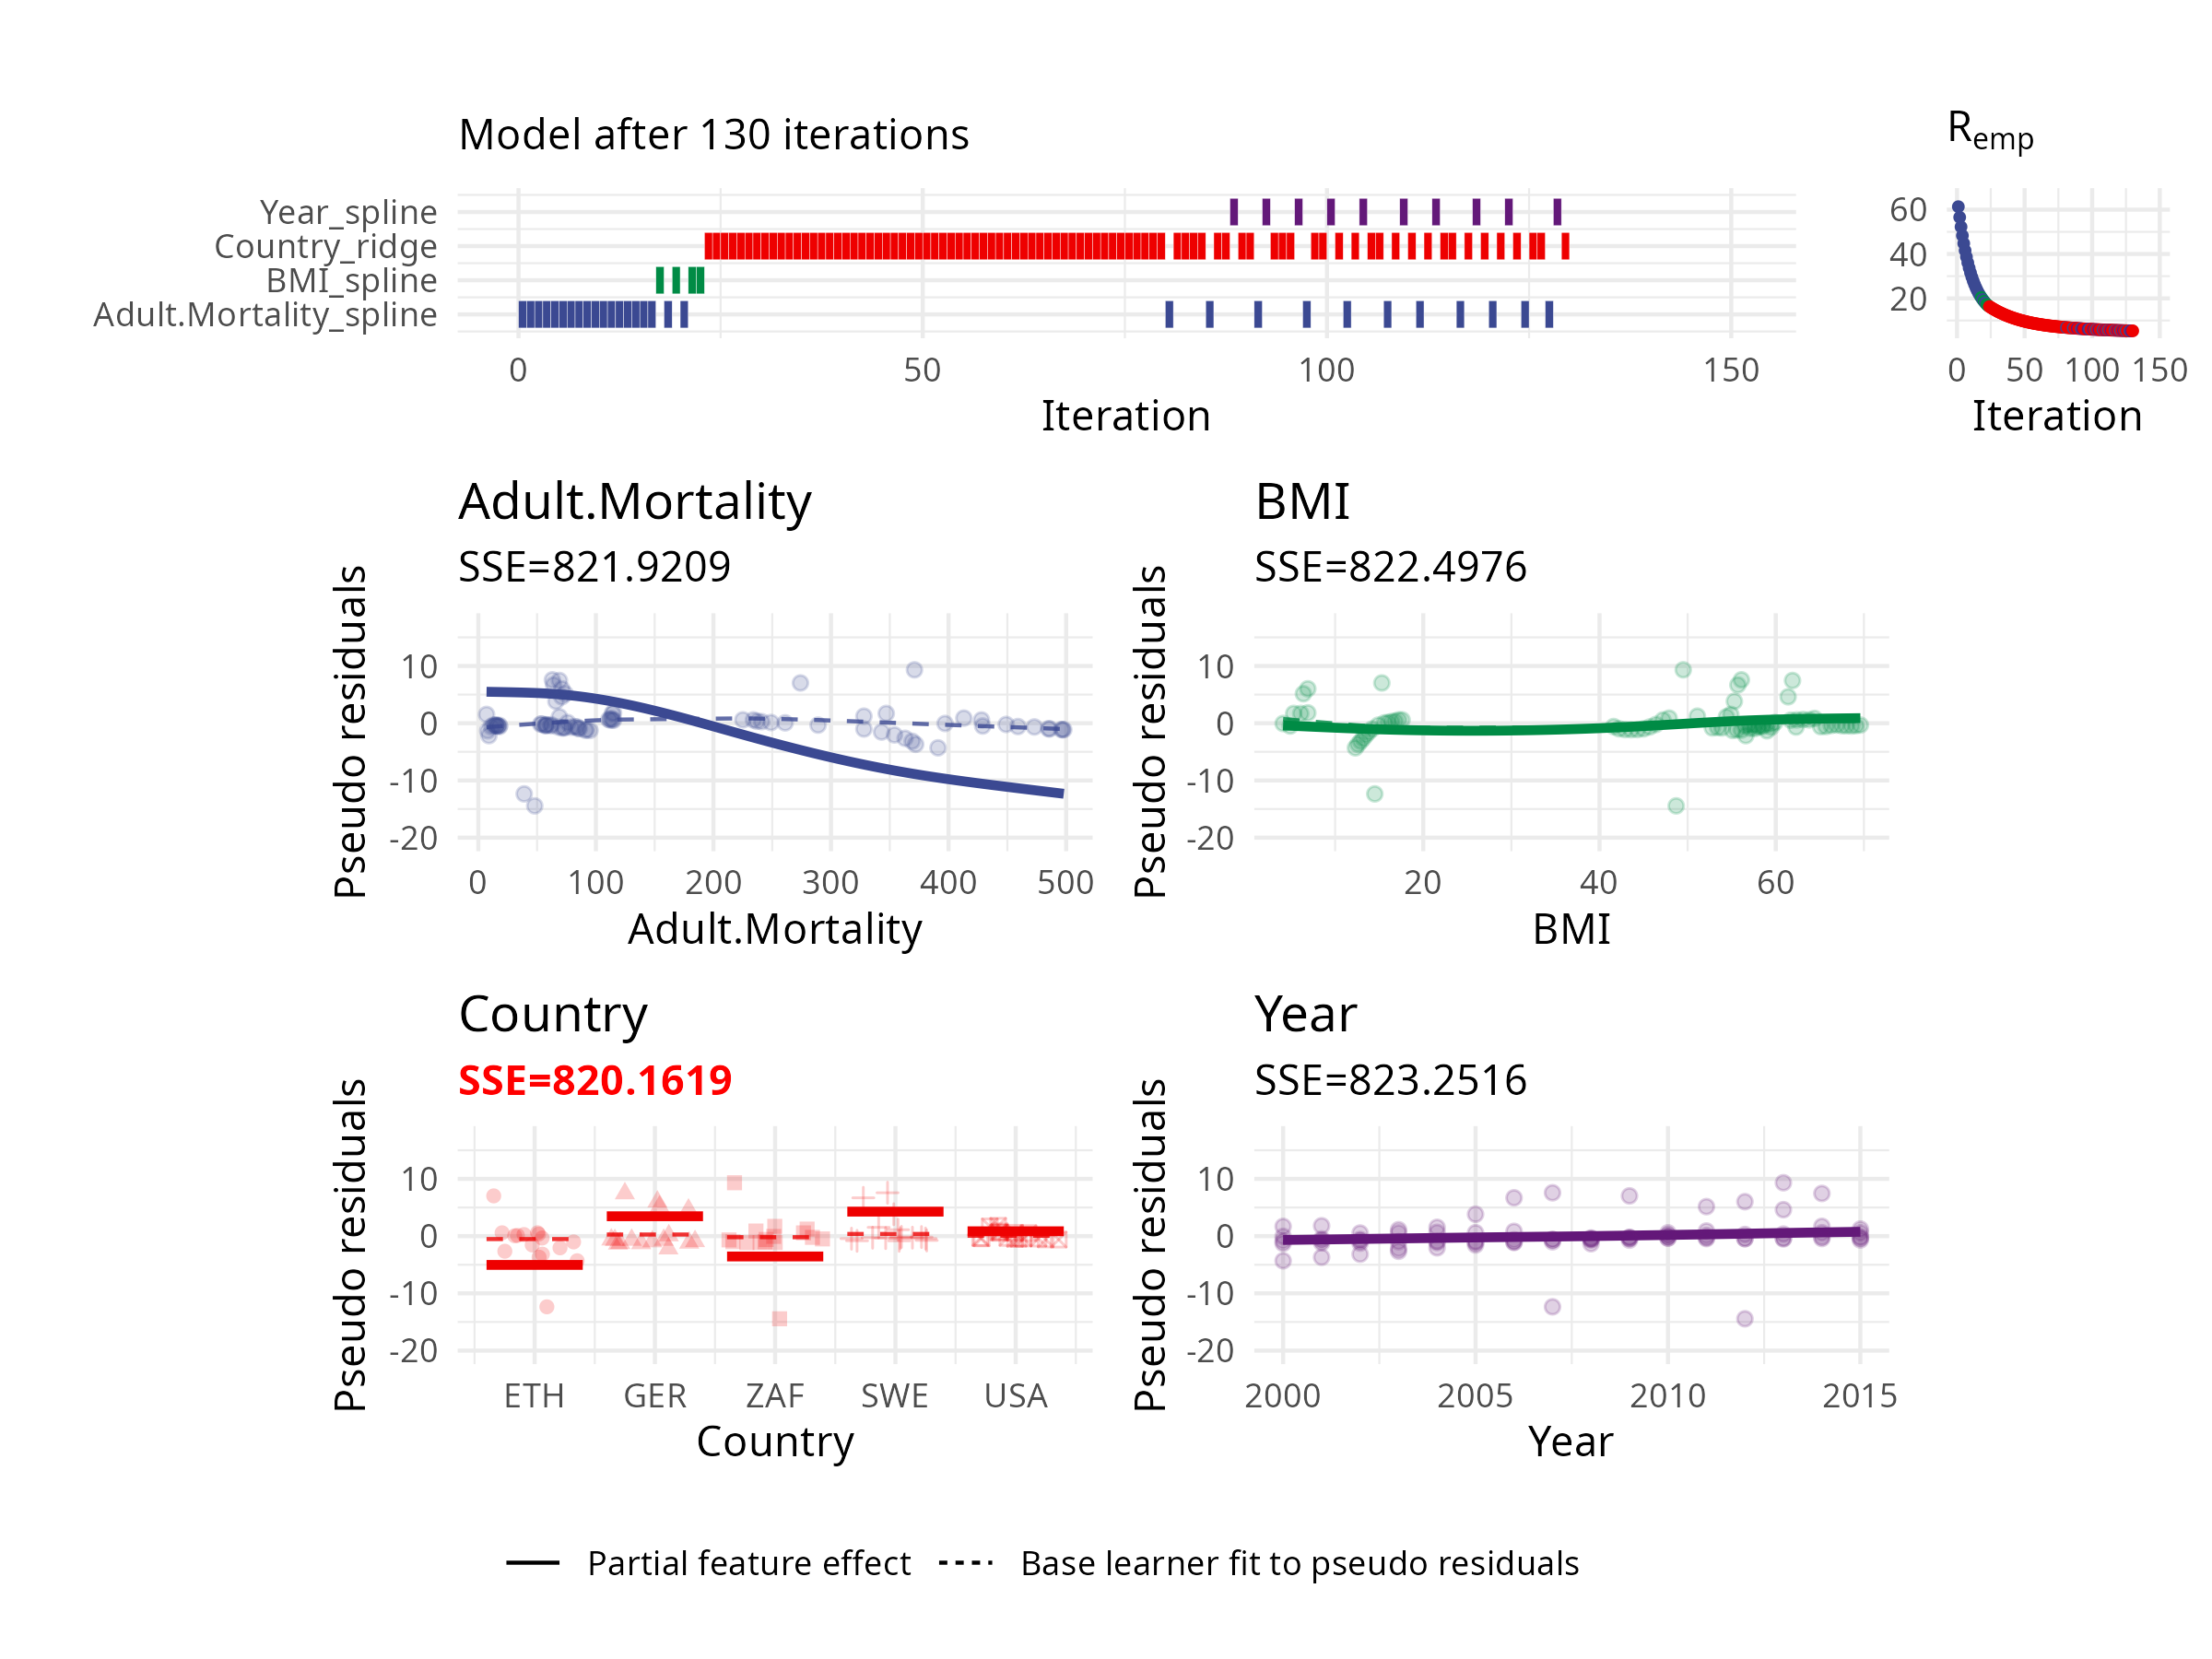
\includegraphics[width=\textwidth]{/home/daniel/repos/diss-presentation/figures/fig-iter-0130.png}
	\end{figure}
	\addtocounter{framenumber}{-1}
\end{frame}


\begin{frame}{Component-wise gradient boosting -- Example}
	\begin{figure}
		\centering
		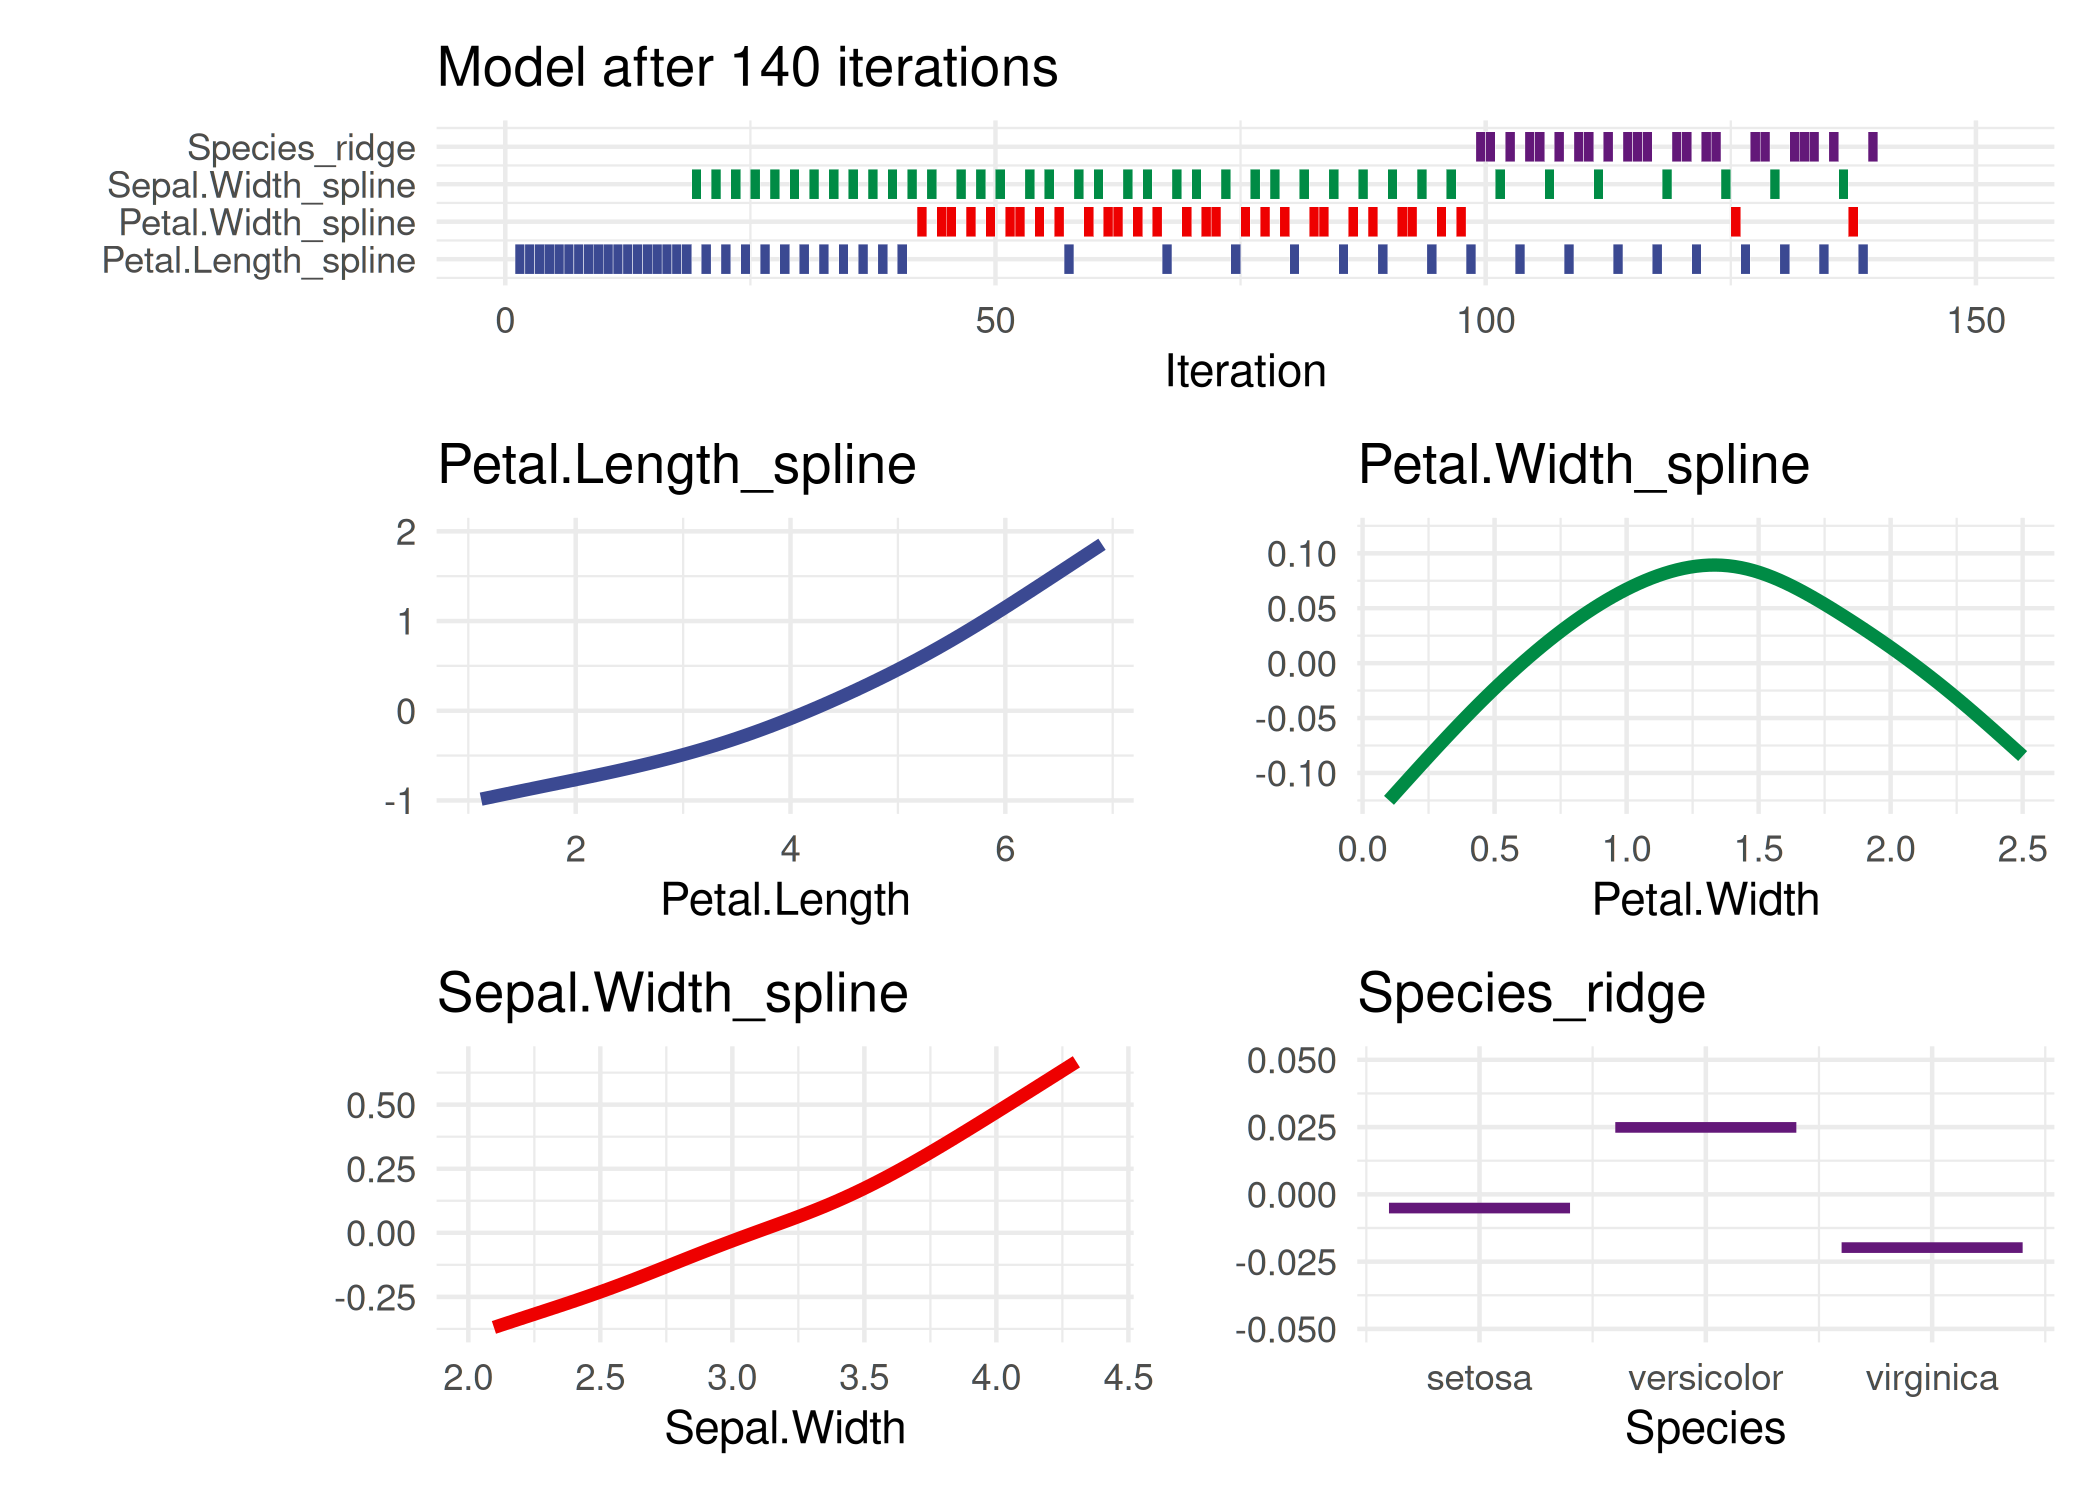
\includegraphics[width=\textwidth]{/home/daniel/repos/diss-presentation/figures/fig-iter-0140.png}
	\end{figure}
	\addtocounter{framenumber}{-1}
\end{frame}


\begin{frame}{Component-wise gradient boosting -- Example}
	\begin{figure}
		\centering
		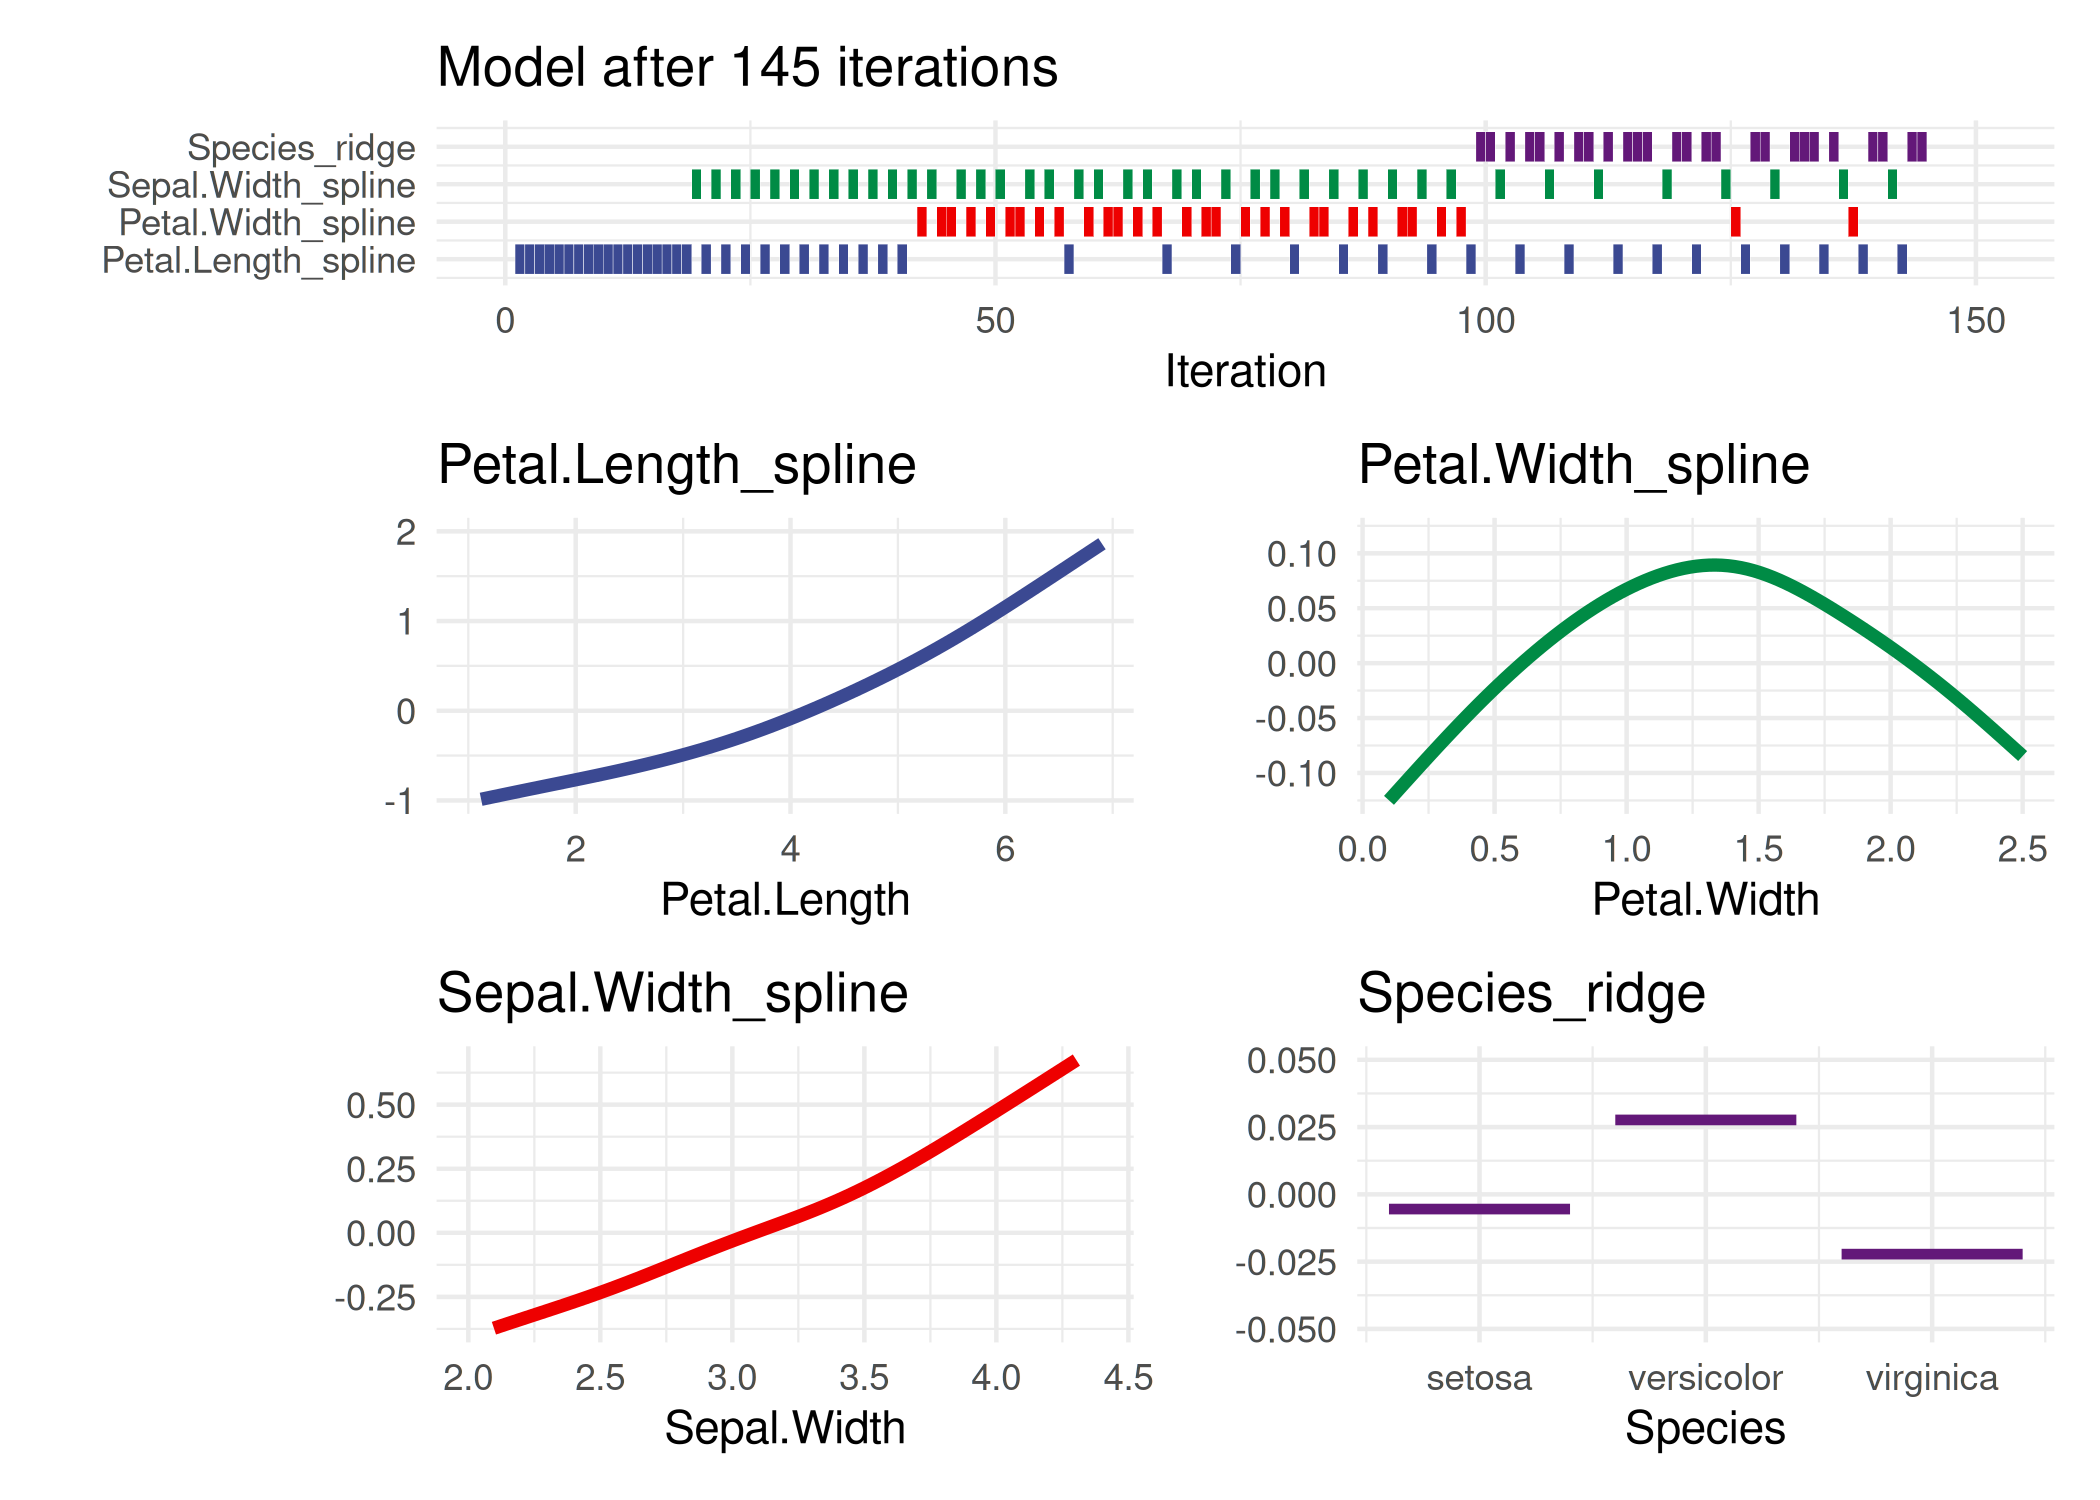
\includegraphics[width=\textwidth]{/home/daniel/repos/diss-presentation/figures/fig-iter-0145.png}
	\end{figure}
	\addtocounter{framenumber}{-1}
\end{frame}


\begin{frame}{Component-wise gradient boosting -- Example}
	\begin{figure}
		\centering
		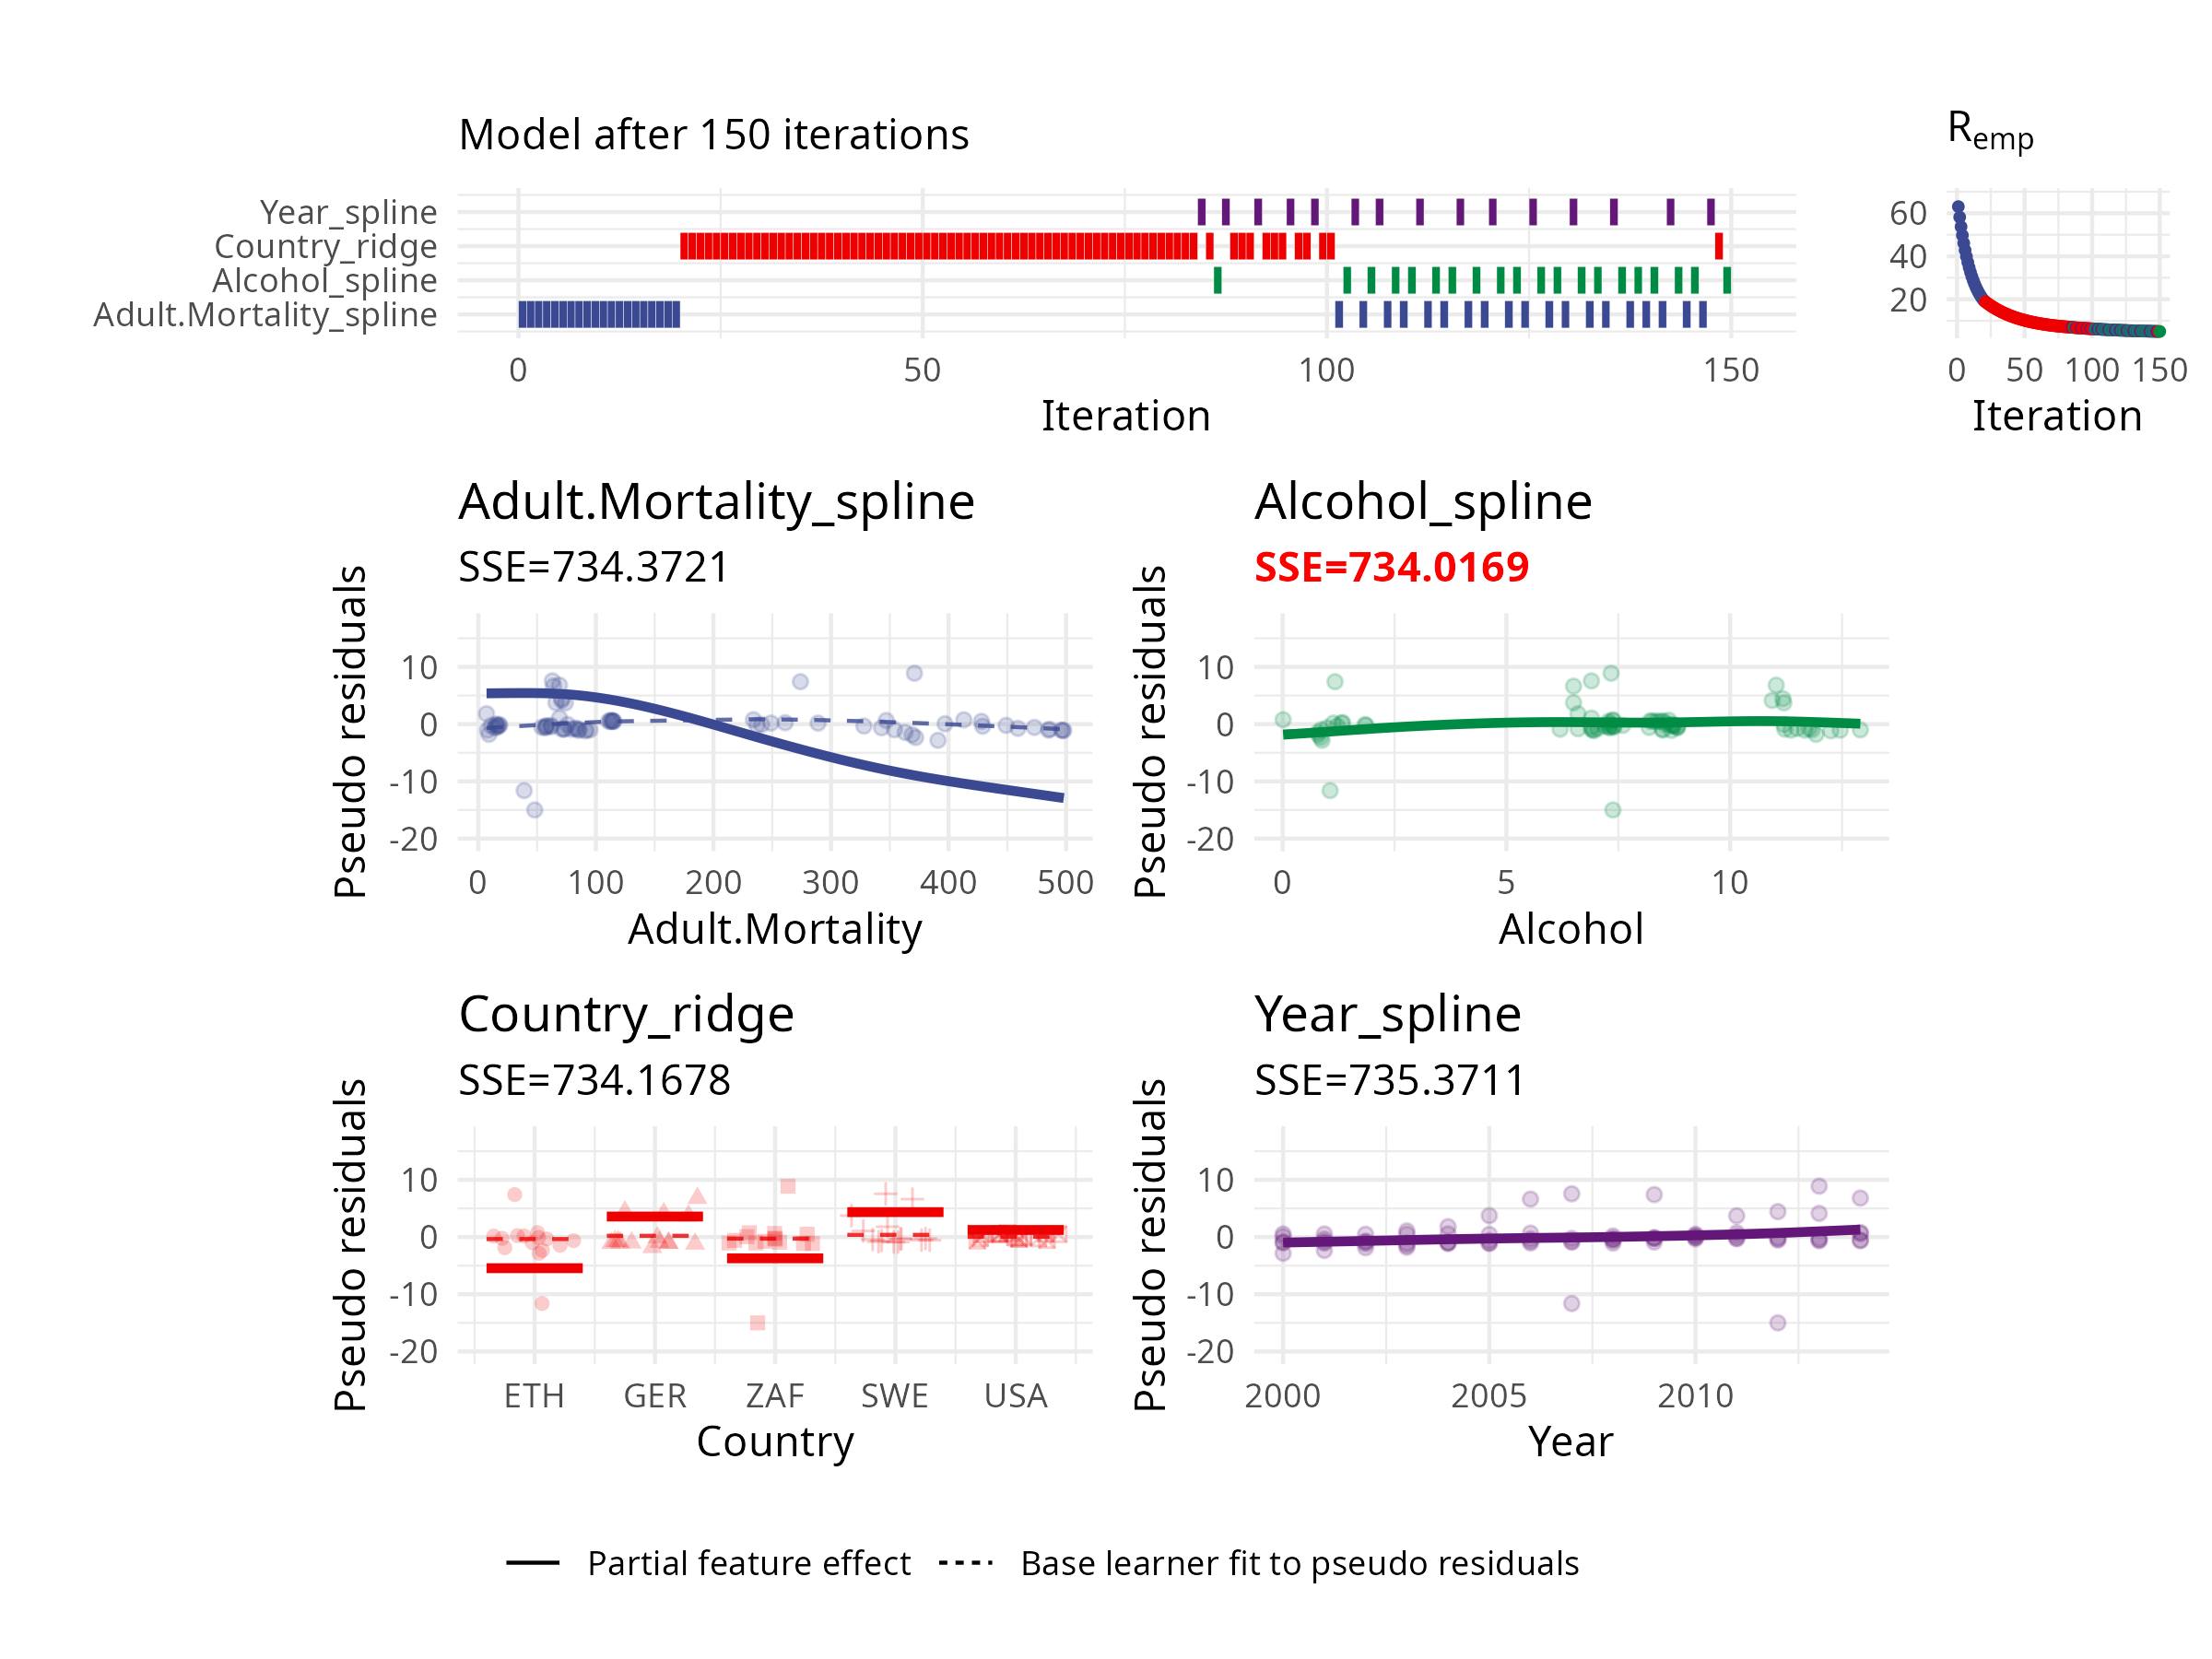
\includegraphics[width=\textwidth]{/home/daniel/repos/diss-presentation/figures/fig-iter-0150.png}
	\end{figure}
	\addtocounter{framenumber}{-1}
\end{frame}



\section{Efficiency}

\begin{frame}{Efficiency}
  About
\end{frame}

\begin{frame}{Adaption}
  About
\end{frame}

\begin{frame}{Results}
  About
\end{frame}



\section{Automation}

\begin{frame}{Automation}
  About
\end{frame}

\begin{frame}{Autocompboost}
  About
\end{frame}

\begin{frame}{Results}
  About
\end{frame}

\begin{frame}{Outlook}
  About
\end{frame}


\section{Distributed computing}

\begin{frame}{Distributed computing}
  About
\end{frame}

\begin{frame}{Adaption}
  About
\end{frame}

\begin{frame}{Results}
  About
\end{frame}

\begin{frame}{Outlook}
  About
\end{frame}


\begin{frame}[allowframebreaks]{Bla}

  Bla
  \citep[see, e.g.,][]{Pepe2003}, or \cite{delong1988comparing}

\end{frame}

\appendix

\begin{frame}[allowframebreaks]{References}

\nocite{*}
\scriptsize
\bibliography{references}

\end{frame}

\section{Backup slides}

\begin{frame}{Backup}

bla

\end{frame}

\end{document}
